\chapter{Hamiltonian Systems with Symmetry} \label{chap:poisson}
%
The geometric exact Cosserat rod formulation preserves symmetries which are exploited throughout this thesis. On choosing suitable constitutive relations the energy-density through the rod is conserved and the governing equations become Hamiltonian. Thus, the geometric formulation allows for a vast array of analytical and numerical tools to be applied. In this chapter the analytical tools which are applied are introduced and placed in the context of rod theory. For a more detailed description of Hamiltonian systems, see for example Arnol'd~\cite{Arnold89} or Olver~\cite{Olver93}.
%
\section{Hamiltonian Systems} \label{sec:lie_poisson}
%
\par
The consequences of the geometrically exact model appear in the Hamiltonian formulation. The equations are naturally noncanonical equations and furthermore the governing equations are Lie-Poisson equations. In this section the Hamiltonian framework is briefly outlined. 
%
\par
The Lie algebra generated by a Lie group $G$ is denoted by $\mathfrak{g}$. The Lie algebra then defines a dual space, $\mathfrak{g}^{*}$, which although is not necessarily a Lie algebra is a vector space. The structure on $\mathfrak{g}$ does not define the structure on its dual other than say that it lies on a Poisson manifold. A Poisson manifold is defined via a Poisson bracket.
%
\begin{defin} \label{def:bracket}
Let $\mathcal{M}$ be a smooth $m$-dimensional manifold, then for any smooth real-valued functions $f$, $g$ and $h$ on $\mathcal{M}$, that is $f$, $g$, $h \in C^{\infty}\left(\mathcal{M}\right)$, the Poisson bracket defines another smooth real-valued function on $\mathcal{M}$ with the following properties
\begin{itemize} \addtolength{\itemsep}{-0.4\baselineskip}
\item[(i)] Bilinearity$\mathrm{:}$ $\{ \alpha f + \beta g , h \} = \alpha \{f,h\} + \beta \{ g, h\}, \quad \forall \, \alpha, \beta \in \mathbb{R}$.
\item[(ii)] Skew-Symmetry$\mathrm{:}$ $\{ f,g \}+\{g,f\}=0$.
\item[(iii)] Jacobi's Identity$\mathrm{:}$ $\{f,\{g,h\}\} + \{h,\{f,g\}\} + \{g,\{h,f\}\} = 0$. 
\item[(iv)] Liebniz's Rule$\mathrm{:}$ $\{f \circ g,h\} = g \circ \{f,h\} + f \circ \{g,h\}$.
\end{itemize}
If the manifold has a Poisson bracket then the manifold is called a Poisson manifold.
\end{defin}
%
Thus a Poisson manifold has a Poisson bracket. A Lie-Poisson bracket is a Poisson bracket created from a Lie algebra.
% 
\begin{defin} \label{def:lie_poisson}
A Lie-Poisson bracket is of the form
\begin{align}
\left\{ f, g \right\}_{\left(\mu\right)} & = \left< \mu, \left[ \frac{\delta f}{\delta \mu}, \frac{\delta g}{\delta \mu} \right] \right> \label{eq:lie_poisson}.
\end{align}
where $\mu \in \mathfrak{g}^{*}$ and $f$, $g$ $\mathrm{:}$ $\mathfrak{g}^{*} \mapsto \mathbb{R}$, with an associated inner product $\left< \cdot, \cdot \right>$ and Lie bracket on the Lie algebra, $\left[ \cdot, \cdot \right]$.  The inner product associates elements of the Lie algebra with its dual and the Lie bracket acts on the function derivatives of $f$ and $g$ with respect to the field variable, that is $\delta f \slash \delta \mu$ $\mathrm{:}$ $\mathfrak{g}^{*} \mapsto \mathfrak{g}$. 
\end{defin}
%
\par
It has been shown that an equation of the form~\eqref{eq:lie_poisson} will satisfy a variational principle~\cite{Bloch96}. Although a Poisson manifold is not necessarily a symplectic manifold it is, however, foliated by collection of submanifolds which are symplectic. Thus
%
\begin{thm}[Darboux' Theorem] \label{thm:reduction}
Let $\mathcal{M}$ be a smooth $m$-dimensional Poisson manifold of constant rank $2n \le m$ everywhere. At each $x_{0} \in \mathcal{M}$ there exist canonical local coordinates $\left( q, p, z \right) = \left(q_{1}, \dots, q_{n}, p_{1}, \ldots, p_{n}, z_{1}, \ldots z_{k} \right)$, where $2n + k = m$, in terms of which the Poisson bracket takes the form
\begin{align}
\left\{ f, g \right\}_{\left(q,p\right)} & = \sum_{i=1}^{n}\left( \frac{\partial f}{\partial q_{i}}\frac{\partial g}{\partial p_{i}} - \frac{\partial f}{\partial p_{i}}\frac{\partial g}{\partial q_{i}} \right). \label{eq:canonical}
\end{align}
\end{thm}
%
\begin{proof}[Proof of \ref{thm:reduction}] 
See~\cite[\S{6.22}]{Olver93}.
\end{proof}
% 
The Poisson bracket~\eqref{eq:canonical} is called the canonical bracket. From the variational structure endowed by the Poisson bracket the Hamiltonian structure can be defined. 
% 
\begin{prop} \label{prop:variational}
The following are equivalent
\begin{itemize}\addtolength{\itemsep}{-0.4\baselineskip}
\item[(iv)] Poisson bracket formulation,
\item[(iii)] Hamilton's equations of motion,
\item[(ii)] Hamilton's principle of stationary action,
\item[(i)] Lagrangian formulation.
\end{itemize}
\end{prop}
% 
\begin{proof}[Proof of \ref{prop:variational}] 
See~\cite{Bloch96}.
\end{proof}
% 
Classically the Hamiltonian is defined from the Legendre transform of the Lagrangian and is the total energy of the system. In the context of rod theory the static equilibria are non-canonical Hamiltonian equations. The governing equations can be constructed in one of either two ways: the static equilibria can be derived from first principles or through the construction of a Lagrangian from the energy stored in the rod and the work done against tension.
% 
\begin{defin} \label{def:hamiltonian}
Let $\mathcal{M}$ be an $m$-dimensional Poisson manifold and let the Hamiltonian be a smooth function such that $\mathcal{H}\left(q,p,z\right): \mathcal{M} \mapsto \mathbb{R}$. The Hamiltonian vector field is the unique, smooth vector field on $\mathcal{M}$ satisfying
\begin{align}
\frac{\mathrm{d}f}{\mathrm{d}t} & = \left\{ f, \mathcal{H}\right\} \nonumber 
\end{align} 
for every smooth function $f\left(q,p,z\right):\mathcal{M}\mapsto\mathbb{R}$. The governing equations are referred to as Hamilton's equations. When the bracket is the canonical bracket~\eqref{eq:canonical}, the governing equations are referred to as Hamilton's canonical equations
\begin{equation}
q^{\prime}= \frac{\partial\mathcal{H}}{\partial p}, \quad  q^{\prime} = -\frac{\partial\mathcal{H}}{\partial q} \quad \mbox{and} \quad z^{\prime} = 0. \nonumber
\end{equation}
\end{defin}
% 
In rod mechanics the Hamiltonian is the total energy density along the rod.
% 
\begin{defin} \label{def:integral}
A function, $f$, is an integral of a Hamiltonian system if it is constant for all solutions of the system. This is equivalent to being in involution with the Hamiltonian, i.e. $ \{ f,\mathcal{H} \} = 0$. Functions which are in involution with every function in the phase space are called Casimir functions. They too are conserved quantities since they are in involution with the Hamiltonian.
\end{defin}
%
\par
Casimirs only exist in non-canonical formulations. In finite-dimensional Hamiltonian systems Casimirs can be found in systematic way~\cite{HernandezBermejo98}. There is a distinction between Casimirs and first integrals. 
%
\begin{description}\addtolength{\itemsep}{-0.4\baselineskip}
\item[First integrals] or nontrivial integrals, are conserved quantities which are dependent on the parameters of the system. In the context of rod theory the first integrals are dependent on the constitutive relations. The Hamiltonian and the integrals of Lagrange and Kovalevskaya, cf.~\eqref{eq:lagrange} and~\eqref{eq:kov} are examples of first integrals in rod theory. They are rare, often difficult to find and may not have an intuitive physical meaning. In some case, such as the Chaplygin-Goryachev integral, cf.~\eqref{eq:chaplygin}, maybe dependent on the values of the Casimirs as well as the parameters of the system. 
\item[Casimirs] or distinguished functions are integrals which are independent of the specific Hamiltonian function but are dependent on the equilibrium equations.  Examples of Casimirs in rod theory are the conservation of the applied moment about the loading axis~\eqref{eq:kirchhoff_casimir1} or the conservation of the magnitude of force force in the body~\eqref{eq:kirchhoff_casimir2} for a rod under end force and torque. Casimirs may be expressed as functions of parameters, see~\eqref{eq:mag_casimir1}, but are not dependent on them.
\item[Subcasimirs] are Casimirs of a substructure matrix or Casimirs of a structure matrix with a constraint, they are independent of the parameters of the system but are dependent on  the values of the Casimirs. Examples of subcasimirs in rod theory are the conservation of curvature in helices for the Kirchhoff rod~\eqref{eq:helix_subcasimirs}.
\end{description}
%
In a sense first integrals are analytic, based on the form of the Hamiltonian, while Casimirs are geometric integrals, based on the structure of the Poisson manifold. In the context of rod theory first integrals are dependent on the material properties of the rod and the Casimirs are dependent on the equilibrium equations.
%
\par
Knowledge of the conserved quantities allows for the equations to be classified as integrable or nonintegrable. In the context of finite dimensional Hamiltonian systems complete integrability is defined as
%
\begin{defin} \label{def:integrability}
A $m$-dimensional Hamiltonian system is said to be completely integrable in the sense of Liouville if it possesses $k$ Casimirs and $n$ first integrals where
\begin{align}
2n + k & = m. \label{eq:count}
\end{align}
Additionally an $m$-dimensional system is superintegrable if $2n + k > m$, minimally superintegrable if it possesses $2n + k = m-1$ integrals and maximally superintegrable if $2n + k = 2m-1$. 
\end{defin}
%
The algebraic and geometric properties of integrability are given by the Arnol'd-Liouville Theorem.
%
\begin{thm}[Arnol'd-Liouville Integrability]\label{thm:arnold-liouville} 
Let an $m$-dimensional Hamiltonian vector field be completely integrable with $k$ Casimirs and $n$ first integrals. Thus the Casimirs induce a canonical Hamiltonian system on the $n$-dimension reduced phase space. Then
\begin{itemize} \addtolength{\itemsep}{-0.5\baselineskip}
\item[(i)] The level set of all first integrals is a manifold which is invariant under the flow of the Hamiltonian.
\item[(ii)] If the manifold is compact and connected then it is diffeomorphic to an $n$-dimensional torus.
\item[(iii)] The phase flow on the torus is `conditionally periodic' on the values of the integrals, both the first integrals and the Casimirs. That is, a unique set of action-angle variables $\left(I,\varphi\right)$ exist.
\item[(iv)] The canonical equations can be integrated by quadrature.
\end{itemize}
\end{thm}
%
\begin{proof}[Proof of \ref{thm:arnold-liouville}] 
See~\cite[pg. 271]{Arnold89}.
\end{proof}
%
The existence of action-angle variables shows that a system is solvable by quadrature, although for practical purposes it is often an existence theorem only. However, integrability has dynamical consequences: the action-angle formulation creates a set of symplectic coordinates $\left(I, \varphi\right)$ such that the actions depend on the integrals and the angles are angular coordinates that flow linearly on the $n$-torus. Thus the Hamiltonian is a function of the actions only. Hence Hamilton's equations are
%
\begin{equation}
{I}^{\prime} = -\dfrac{\partial \mathcal{H}}{\partial \varphi} \quad \mbox{and} \quad {\varphi}^{\prime} = \dfrac{\partial \mathcal{H}}{\partial I}.
\end{equation} 
%
It follows that
%
\begin{equation}
{I}^{\prime} = 0 \quad \mbox{and} \quad {\varphi}^{\prime} = \omega \label{eq:action_angle}
\end{equation}
%
where $\omega$ are the frequencies of the motion on the torus and
%
\begin{align}
I & = I\left( h, p \right) \quad \mbox{such that} \quad I_{i} = \dfrac{1}{2\pi}\oint_{ \gamma_{i} } p_{i} \, \mathrm{d}q_{i} \quad i=1,\ldots,n \nonumber
\end{align}
%
over cycles $\gamma_{i}$.  
%
\par
If the independent integrals do not form a compact and smooth manifold then the system is said to have monodromy. This prohibits the construction of global action-angle coordinates. 
%
\par
As mentioned, if the principal bending stiffnesses of a rod under end tension and moment are equal then the governing equations are completely integrable. Thus all configurations can be expressed in closed form. However a global set of action-angle variables cannot be created on every energy level~\cite{Cushman85}. If a global set of action-angle variables can be created on an energy level the singular fibrations of the torus define the bifurcation values.
% 
\begin{defin} \label{def:nondegenerate}
An integrable system is said to be non-degenerate if  
\begin{align}
\left| \dfrac{\partial \omega}{ \partial I} \right| = \left| \dfrac{\partial^{2} \mathcal{H}}{ \partial I^{2}} \right| & \ne 0. \nonumber
\end{align}
\end{defin}
%
\noindent
A simple way of creating a degenerate system is to have a pair of resonant frequencies $\omega_{i}=\omega_{j}$ with $i \ne j$. 
%
\begin{lem} \label{lem:uniqueness_tori}
If a system is non-degenerate then the invariant tori are uniquely defined and independent of the choice of action-angle coordinates.
\end{lem} 
%
\begin{proof}
See~\cite[pg. 290]{Arnold89}.
\end{proof} 
%
The definition of degeneracy relates the dependence of the Hamiltonian to the action integrals and primarily relates to the time scales in which perturbations effect the system in \textsc{kam} theory. However, in this study it shall be shown that the nondegeneracy condition plays a role in defining the order of the perturbation in a canonical Hamiltonian system.
%
\par
The main benefits of action-angle coordinates are that they allow insight into the bifurcation structure of a system and through perturbation analysis can shed light on the behaviour of nonintegrable systems nearby.
%
\section{Mel'nikov's Theory} \label{sec:melnikov_thm}
%
Most naturally occurring systems are nonintegrable, however many can be considered to be perturbations of integrable systems. For rod theory, some perturbations such as extensibility and a force due to a magnetic field do not destroy integrability while others such as anisotropy and initial curvature do destroy integrability through the loss of a first integral. In this section Mel'nikov's theory is introduced and an instructive example presented.
%
\par
The Mel'nikov integral~\cite{Melnikov63,Holmes83} is used to analyse a perturbation of a homoclinic orbit in an integrable Hamiltonian systems, giving a measure (to first order) of the distance between the unstable and stable manifolds of the perturbed homoclinic, as is illustrated in figure~\ref{fig:Mel}. If the Mel'nikov integral has simple zeroes then the stable and unstable perturbed homoclinic manifolds intersect transversely. Devaney's theorem~\cite{Devaney78} states that if the perturbation yields a transverse intersection of the stable and unstable manifolds then the existence of an associated transverse homoclinic orbits allows, via the Smale-Birkhoff theorem, horseshoes on the Poincar\'e sections of the level sets defined by the homoclinic energy. In turn, the system is no longer integrable. Given the transversal intersection of the stable and unstable manifolds there then exists configurations with arbitrarily high period which are embedded in an invariant Cantor set. Hence, there exists a multiplicity of multimodal homoclinic solutions~\cite{Belyakov90} and~\cite[\S{2.4.1}]{Guckenheimer83}. 
% 
\begin{figure}[!htbp]
\begin{center}
%GNUPLOT: LaTeX picture with Postscript
\begin{picture}(0,0)%
\includegraphics{Images/epslatex/Melnikov.eps}%
\end{picture}%
\begingroup
\setlength{\unitlength}{0.0200bp}%
\begin{picture}(18000,10800)(0,0)%
\put(15385,8116){\makebox(0,0)[l]{\strut{}$f_{0}\left(\boldsymbol{x}_{0} \left(0\right) \right)$}}%
\put(12998,10250){\makebox(0,0)[l]{\strut{}$f_{0}\left(\boldsymbol{x}_{0} \left(0\right) \right)^{\perp}$}}%
\put(13819,9400){\makebox(0,0)[l]{\strut{}$q_{\epsilon}^{u} \left(\varphi_{0}\right)$}}%
\put(12743,6979){\makebox(0,0)[l]{\strut{}$q_{\epsilon}^{s} \left(\varphi_{0}\right)$}}%
\put(3984,3266){\makebox(0,0)[l]{\strut{}$W_{\epsilon}^{s}\left( \boldsymbol{p}_{\epsilon}^{\varphi_{0}} \right)$}}%
\put(4233,7728){\makebox(0,0)[l]{\strut{}$W_{\epsilon}^{u}\left( \boldsymbol{p}_{\epsilon}^{\varphi_{0}} \right)$}}%
\put(3093,5400){\makebox(0,0)[l]{\strut{}$\boldsymbol{p}$}}%
\put(825,5400){\makebox(0,0)[l]{\strut{}$\boldsymbol{p}_{\epsilon}^{\varphi_{0}}$}}%
\put(2257,9280){\makebox(0,0)[l]{\strut{}$\Sigma^{\varphi_{0}}$}}%
\end{picture}%
\endgroup
\endinput
 
\end{center}
\vspace*{-1.0cm}
\caption[Schematic diagram of Mel'nikov's method]{\baselineskip=1.0\normalbaselineskip% 
Schematic illustration of Mel'nikov's method on a Poincar\'e section $\Sigma_{}^{\varphi_{0}}$ showing the distance between the perturbed stable $W^{s}_{\epsilon}$ (light blue) and unstable manifolds $W^{s}_{\epsilon}$ (dark blue) of a homoclinic $\boldsymbol{x}_{0}\left(\varphi\right)$ (dotted) at a point $\varphi_{0}$. Note that $\boldsymbol{p}$ is a fixed point but $\boldsymbol{p}_{\epsilon}^{\varphi_{0}}$ is a periodic orbit with a fixed point on the Poincar\'e map $\Sigma_{}^{\varphi_{0}}$. \label{fig:Mel} }
\end{figure}
%
\par
Mel'nikov's original theorem needs to be adapted when the unperturbed phase space is comprised of a pair of canonical variables with symmetry properties. Let the perturbed system take the form
%
\begin{align}
\mathcal{H}_{\epsilon}\left(q,p,\varphi,I\right) & = \mathcal{H}_{0}\left(q,p,I\right) + \epsilon \mathcal{H}_{1}\left(q,p,\varphi,I\right) + \mathcal{O}\left( \epsilon^{2}\right) \label{eq:perturbed_hamiltonian}
\end{align}
%
where the unperturbed integrable Hamiltonian system is given by the two-dimensional system
%
\begin{align}
\mathcal{H}_{0} & = \mathcal{H}_{0}\left( q, p, I \right)
\end{align}
%
on the energy level $h$. In order for the analysis to hold in a Lie-Poisson system, two assumptions need to be satisfied:
%
\begin{itemize}\addtolength{\itemsep}{-0.5\baselineskip}
\item[({H1})] The unperturbed Hamiltonian system possesses a homoclinic orbit of the form
\begin{align}
\boldsymbol{x}_{0}\left(s\right) &= \left( q\left(s;h\right), p\left(s;h\right) \right) \nonumber 
\end{align}
to a hyperbolic fixed point
\begin{align}
\boldsymbol{p} = \boldsymbol{x}_{0}\left(0\right) &= \left( q\left(0;h\right), p\left(0;h\right) \right) \nonumber 
\end{align}
for each $h$ in an interval $h \in J^{h} \subset \mathbb{R}$, where the interval $J^{h}$ is the set of energy levels which admit homoclinic orbits. The homoclinic depends on the energy level via the action $I_{h}=I\left(h\right)$ corresponding to the homoclinic orbit and the total energy $\mathcal{H}_{0}\left(x_{0},I\right)=h$.
\item[({H2})] For $h \in J^{h} $ and $\boldsymbol{x}_{0}$ the frequency
\begin{align}
\omega_{0} & = \omega_{0}\left( \boldsymbol{x}_{0}, I_{h} \right) = \dfrac{\partial \mathcal{H}_{0}}{\partial I} \label{eq:Omega_0} 
\end{align}
of the unperturbed system satisfies the condition $\left| \omega_{0} \right| \ge \delta > 0$ for some $\delta \in \mathbb{R}^{+}$ and $\forall s \in\left(-\infty,+\infty\right)$. Thus
\begin{align}
\varphi\left(s\right) & = \varphi_{0} + \int^{s}\omega_{0}\left(\bar{s}\right)\,\mathrm{d}\bar{s} = \varphi_{0} + \bar{\varphi}\left(s\right)
\end{align}
and  
\begin{align}
\lim_{s\rightarrow\pm\infty} \varphi\left(s\right) & = \pm \infty.
\end{align}
\end{itemize}
%
% In a general system $\omega_{0}$ would be a constant, but in a Lie-Poisson system as there is a coupling in the unperturbed Hamiltonian between the actions and the conjugates, i.e., $\mathcal{H}_{0}\left(q\left(s\right),p\left(s\right),I\right)$ then $\omega_{0} = \omega_{0}\left(s\right)$.
%
\par
By the first condition~({H1}), the unperturbed Hamiltonian may be inverted and solved for $I_{h}$ up to order $\epsilon$. By the second condition~({H2}), $\varphi$ can be treated as a `time-like' variable. By the Implicit Function Theory, the (constant) action $I_{h}$ is denoted by the expansion
%
\begin{align}
I_{h} & = I_{h}\left(q,p,\varphi\right) =  I^{\left(0\right)} + \epsilon I^{\left(1\right)} + \mathcal{O}\left(\epsilon^{2}\right). \label{eq:act_expansion}
\end{align}
%
The derivative of the angle coordinate, i.e. the frequency on the torus, can be expanded for small $\epsilon$
%
\begin{align}
{\varphi}^{\prime} = \dfrac{\partial \mathcal{H}_{\epsilon}}{\partial I} & = \omega_{\epsilon} \nonumber \\
& = \omega_{0} + \epsilon \dfrac{\partial \mathcal{H}_{1}}{\partial I} + \mathcal{O}\left(\epsilon^{2}\right). \label{eq:simple1}
\end{align}
%
As
%
\begin{align}
\dfrac{\partial \mathcal{H}}{\partial p} & = \dfrac{\mathrm{d}q}{\mathrm{d}\varphi}\dfrac{\mathrm{d}\varphi}{\mathrm{d}t} \quad \mbox{and} \quad \dfrac{\partial \mathcal{H}}{\partial q} = -\dfrac{\mathrm{d}p}{\mathrm{d}\varphi}\dfrac{\mathrm{d}\varphi}{\mathrm{d}t} \label{eq:simple2}
\end{align} 
% 
then from~\eqref{eq:simple1} and~\eqref{eq:simple2} the following relationships hold
%
\begin{equation} \label{eq:new_time}
\dfrac{\mathrm{d}q}{\mathrm{d}\varphi} =  \omega_{\epsilon}^{-1} \dfrac{\partial \mathcal{H}_{\epsilon}}{\partial p} \quad \mbox{and} \quad \dfrac{\mathrm{d}p}{\mathrm{d}\varphi} = -\omega_{\epsilon}^{-1} \dfrac{\partial \mathcal{H}_{\epsilon}}{\partial q}.
\end{equation} 
%
Given $h = \mathcal{H}_{\epsilon}$ then implicit differentiation of $\mathcal{H}_{\epsilon}\left( q, p, I\left(q,p,\varphi\right),\varphi\right)$ with respect to both canonical coordinates $\left(q,p\right)$ at the homoclinic energy level yields
%
\begin{equation} \label{eq:new_ham}
\dfrac{\partial \mathcal{H}_{\epsilon}}{\partial q} + \omega_{\epsilon}\dfrac{\partial I_{h}}{\partial q} = 0 \quad \mbox{and} \quad \dfrac{\partial \mathcal{H}_{\epsilon}}{\partial p} + \omega_{\epsilon}\dfrac{\partial I_{h}}{\partial p} = 0. 
\end{equation}
%
It follows from~\eqref{eq:new_time} and~\eqref{eq:new_ham} that
%
\begin{equation}
\frac{\mathrm{d}q}{\mathrm{d}\varphi} = - \dfrac{\partial I_{h}}{\partial p} \quad \mbox{and} \quad \frac{\mathrm{d}p}{\mathrm{d}\varphi} =  \dfrac{\partial I_{h}}{\partial q}.
\end{equation}
%
The angle coordinate on the torus, $\varphi$, now plays the role of time in a new Hamiltonian system, where the Hamiltonian is played by the action, $I_{h}$. In order to find the terms in the expansion of $I_{h}$ in~\eqref{eq:act_expansion} the Hamiltonian is expanded 
%
\begin{align}
h & = \mathcal{H}_{\epsilon}\left(q,p,\varphi,I^{\left(0\right)} + \epsilon I^{\left(1\right)} + \mathcal{O}\left(\epsilon^{2}\right) \right) \nonumber \\
& = \mathcal{H}_{0}\left(q,p,I^{\left(0\right)} + \epsilon I^{\left(1\right)} + \mathcal{O}\left(\epsilon^{2}\right)\right) + \epsilon\mathcal{H}_{1}\left(q,p,\varphi,I^{\left(0\right)} + \epsilon I^{\left(1\right)} + \mathcal{O}\left(\epsilon^{2}\right) \right), \nonumber \\
& = \mathcal{H}_{0}\left(q,p, I^{\left(0\right)}\right) + \epsilon I^{\left(1\right)}\omega_{0}\left(q,p,I^{\left(0\right)}\right) + \epsilon\mathcal{H}_{1}\left(q,p,\varphi,I^{\left(0\right)}\right) + \mathcal{O}\left(\epsilon^{2}\right). \label{eq:ham_expansion}
\end{align}
%
Comparing coefficients of $\epsilon$ for the expansions of the Hamiltonian~\eqref{eq:ham_expansion} with the action~\eqref{eq:act_expansion} to first order yields
%
\begin{subequations}
\label{eq:coeff_matching}
\begin{align}
I_{}^{\left(0\right)}\left(q,p\right) & = \mathcal{H}_{0}^{-1}\left( q, p\right)\left(h\right), \label{eq:coeff_matching0} \\
I_{}^{\left(1\right)}\left(q,p,\varphi\right)  & = - \dfrac{\mathcal{H}_{1}^{}\left( q, p, \varphi, I_{}^{\left(0\right)}\right)}{\omega_{0}^{}\left(q,p,I_{}^{\left(0\right)}\right)} \nonumber \\
& = -\dfrac{\mathcal{H}_{1}^{}\left(q, p, \varphi, \mathcal{H}_{0}^{-1}\left(q,p\right)\left(h\right) \right) }{ \omega_{0}^{}\left(q, p, \mathcal{H}_{0}^{-1}\left(q,p\right)\left(h\right) \right) },\label{eq:coeff_matching1}
\end{align}
\end{subequations}
%
where $\mathcal{H}_{0}^{-1}\left(q,p\right)\left(h\right)$ denotes the inversion of $\mathcal{H}_{0}$ with respect to $I$ at $h$.  Hence Hamilton's equations are
%
\begin{subequations} 
\label{eq:perturbed_vector_field}
\begin{align}
\frac{\mathrm{d}q}{\mathrm{d}\varphi} & = -\dfrac{\partial I^{\left(0\right)}}{\partial p} - \epsilon\dfrac{\partial I^{\left(1\right)}}{\partial p} - \mathcal{O}\left(\epsilon^{2}\right), \\
\frac{\mathrm{d}p}{\mathrm{d}\varphi} & = \dfrac{\partial I^{\left(0\right)}}{\partial q} + \epsilon\dfrac{\partial I^{\left(1\right)}}{\partial q} + \mathcal{O}\left(\epsilon^{2}\right). 
\end{align}
\end{subequations}
%
Using the expressions for $I^{\left(n\right)}$ derived in~\eqref{eq:coeff_matching1}, a $n^{\mathrm{th}}$-order approximation to the governing equations in terms of the unperturbed system can be calculated. The unperturbed vector field is in fact a scaled version of the original problem, that is
%
\begin{align}
\left( -\frac{\partial I^{\left(0\right)}}{\partial p}, \frac{\partial I^{\left(0\right)}}{\partial q} \right) = \frac{1}{\omega_{0}}\left( \frac{\partial \mathcal{H}_{0}}{\partial p}, -\frac{\partial \mathcal{H}_{0}}{\partial q} \right).
\end{align}
%
Thus, if the first condition~({H1}) is satisfied then unperturbed vector field \eqref{eq:perturbed_vector_field} has a hyperbolic fixed point. 
%
\par
It should be noted that to higher orders conditions on the dependence of the Hamiltonian to the action integral appear~\ref{def:nondegenerate} appear. 
% 
\par
For simplicity in the notation let $\boldsymbol{x}=\left(q,p\right)$ and let $f_{i} = \epsilon^{i} \left( -{\partial I_{i}}\slash{\partial p}, {\partial I_{i}}\slash{\partial q} \right)^{T}$. For $u=\left(u_{1},u_{2}\right)$ and $v=\left(v_{1},v_{2}\right)$ the wedge product is defined as
% 
\begin{align}
u \wedge v & = u_{1}v_{2} - v_{1}u_{2}.
\end{align}
% 
Let $Df$ denote the Jacobian of $f$ and $D^{2}f_{0}^{} \,\left(\boldsymbol{x}_{1}^{s,u}\right)^{2}$ be shorthand for $ \left( D\left( D f_{0}^{} \boldsymbol{x}_{1}^{s,u} \right) \right) \boldsymbol{x}_{1}^{s,u}$. 
% 
\begin{thm}[Mel'nikov's Theory]\label{thm:melnikov}
Consider the `time' dependent distance function
\begin{align}
\Delta_{\epsilon}^{}\left(\varphi,\varphi_{0}^{}\right) & = f_{0}^{}\left(\boldsymbol{x}_{0}^{}\left(\varphi-\varphi_{0}^{}\right)\right) \wedge\left( \boldsymbol{x}_{\epsilon}^{u}\left(\varphi,\varphi_{0}^{}\right)-\boldsymbol{x}_{\epsilon}^{s}\left(\varphi,\varphi_{0}^{}\right) \right) \label{eq:mel1}
\end{align}
where $\boldsymbol{x}_{\epsilon}^{u}$ and $\boldsymbol{x}_{\epsilon}^{s}$ are the flows on the stable and unstable perturbed homoclinic manifolds (see appendix~\S\ref{sec:preliminaries} for more detail).  The Mel'nikov function is defined as
\begin{align}
\Delta_{\epsilon}\left(\varphi_{0}\right) &= \Delta_{\epsilon}\left(\varphi_{0},\varphi_{0}\right).
\end{align}
The Mel'nikov function can be expressed as the sum of Mel'nikov integrals
\begin{align}
\Delta_{\epsilon}^{}\left(\varphi_{0}^{}\right) & = \epsilon\mathcal{M}_{h}^{\left(1\right)}\left(\varphi_{0}^{}\right) +\epsilon^{2}\mathcal{M}_{h}^{\left(2\right)}\left(\varphi_{0}^{}\right) + \mathcal{O}\left(\epsilon_{}^{3}\right).
\end{align}
The first order Mel'nikov integral is given by 
% \begin{align}
% \mathcal{M}_{h}^{\left(1\right)}\left(\varphi_{0}\right) & = \int^{+\infty}_{-\infty} \left\{ I_{}^{\left(0\right)}, I_{}^{\left(1\right)} \right\}_{\left(q,p\right)} \, \mathrm{d}\varphi
% \end{align}
\begin{align}
\mathcal{M}_{h}^{\left(1\right)}\left(\varphi_{0}\right) & = \int^{+\infty}_{-\infty} f_{0}^{}\left(\boldsymbol{x}_{0}^{}\left(\varphi-\varphi_{0}^{}\right)\right) \wedge f_{1}^{}\left(\boldsymbol{x}_{0}^{}\left(\varphi-\varphi_{0}^{}\right),\varphi\right) \, \mathrm{d}\varphi
\end{align}
and the second order Mel'nikov integral is given by
\begin{align}
\mathcal{M}_{h}^{\left(2\right)}\left(\varphi_{0}^{}\right) & = \dfrac{1}{2}\!\int_{\varphi_{0}}^{+\infty} f_{0}^{} \wedge D^{2}_{}f_{0}^{}\left(\boldsymbol{x}_{1}^{s}\right)_{}^{2} \,\mathrm{d}\varphi + \dfrac{1}{2}\!\int_{-\infty}^{\varphi_{0}^{}} f_{0}^{} \wedge D^{2}_{}f_{0}^{}\left(\boldsymbol{x}_{1}^{u}\right)_{}^{2} \,\mathrm{d}\varphi \nonumber \\
& \hspace{1.0cm} + \dfrac{1}{2}\!\int_{\varphi_{0}}^{+\infty} f_{0}^{} \wedge Df_{1}^{}\boldsymbol{x}_{1}^{s} \, \mathrm{d}\varphi
+ \dfrac{1}{2}\!\int_{-\infty}^{\varphi_{0}} f_{0} \wedge Df_{1}^{}\boldsymbol{x}_{1}^{u} \,\mathrm{d}\varphi \nonumber \\ 
& \hspace{1.5cm} + \int_{-\infty}^{+\infty} f_{0}^{}\left(\boldsymbol{x}_{0}^{}\left(\varphi-\varphi_{0}^{}\right)\right) \wedge f_{2}^{}\left(\boldsymbol{x}_{0}^{}\left(\varphi-\varphi_{0}^{}\right),\varphi\right) \,\mathrm{d}\varphi. 
\end{align}
Where $\boldsymbol{x}_{1}^{s}\left(\varphi,\varphi_{0}^{}\right)$ are the solutions to a variational equation 
\begin{align}
\dfrac{ \mathrm{d}}{\mathrm{d}\varphi}\boldsymbol{x}_{1}^{s,u} \left(\varphi,\varphi_{0}^{}\right) & = Df_{0}^{}\left(\boldsymbol{x}_{0}^{}\left(\varphi-\varphi_{0}^{}\right)\right)\boldsymbol{x}_{1}^{s,u}\left(\varphi,\varphi_{0}^{}\right) + f_{1}^{}\left(\boldsymbol{x}_{0}^{}\left(\varphi-\varphi_{0}^{}\right),\varphi\right)
\end{align}
subject to the conditions that solutions are bounded and transverse to the flow of the unperturbed homoclinic
\begin{subequations} 
\begin{align}
\left< \boldsymbol{x}_{1}^{s,u}\left(\varphi_{0}^{},\varphi_{0}^{}\right), f_{0}^{}\left( \boldsymbol{x}_{0}^{}\left(\varphi-\varphi_{0}^{}\right)\right) \right> & = 0,  \\
\lim_{\varphi\rightarrow \pm \infty} \big| \left< \boldsymbol{x}_{1}^{s,u}\left(\varphi_{0}^{},\varphi_{0}^{}\right), f_{0}^{}\left( \boldsymbol{x}_{0}^{}\left(\varphi-\varphi_{0}^{}\right)\right) \right> \big| & \le K .
\end{align}
\end{subequations}
The two conditions provide initial conditions so that unique solutions to the first order variational equation can be found. If the Mel'nikov function has simple zeroes then the stable and unstable manifolds intersect transversally for the perturbed system. Conversely, if the Mel'nikov integral is bounded away from zero then the manifolds do not intersect and there are no transverse intersections. 
\end{thm}
%
\begin{proof}[Proof of \ref{thm:melnikov}]
% 
The distance function~\eqref{eq:mel1} can be decomposed into constituent up to second order are
% 
\begin{align}
\Delta_{\epsilon}^{}\left(\varphi,\varphi_{0}^{}\right) & = \Delta_{\epsilon,1}^{-}\left(\varphi,\varphi_{0}^{}\right) - \Delta_{\epsilon,1}^{+}\left(\varphi,\varphi_{0}^{}\right) + \Delta_{\epsilon,2}^{-}\left(\varphi,\varphi_{0}^{}\right) - \Delta_{\epsilon,2}^{+}\left(\varphi,\varphi_{0}^{}\right) + \mathcal{O}\left(\epsilon_{}^{3}\right)
\end{align}
% 
The stable part of the first order term is given by
% 
\begin{align}
\Delta_{\epsilon,1}^{+}\left(\varphi,\varphi_{0}^{}\right) & = f_{0}^{}\left(\boldsymbol{x}_{0}^{}\left(\varphi-\varphi_{0}^{}\right)\right) \wedge \boldsymbol{x}_{1}^{s}\left(\varphi,\varphi_{0}^{}\right).
\end{align}
% 
Similarly, the corresponding second order term is given by
% 
\begin{align}
\Delta_{\epsilon,2}^{+}\left(\varphi,\varphi_{0}^{}\right) & =  f_{0}^{}\left(\boldsymbol{x}_{0}^{}\left(\varphi-\varphi_{0}^{}\right)\right) \wedge \boldsymbol{x}_{2}^{s}\left(\varphi,\varphi_{0}^{}\right).
\end{align}
% 
The derivative of the first order term is
% 
\begin{align}
\dfrac{\mathrm{d}}{\mathrm{d}\varphi}\Delta_{\epsilon,1}^{+}\left(\varphi,\varphi_{0}^{}\right) & = Df_{0}^{}\left(\boldsymbol{x}_{0}^{}\left(\varphi,\varphi_{0}^{}\right)\right) f_{0}^{}\left(\boldsymbol{x}_{0}^{}\left(\varphi-\varphi_{0}^{}\right)\right) \wedge \boldsymbol{x}_{1}^{s}\left(\varphi,\varphi_{0}^{}\right) \nonumber \\
& \hspace{0.5cm} + f_{0}^{}\left(\boldsymbol{x}_{0}^{}\left(\varphi-\varphi_{0}^{}\right)\right) \wedge Df_{0}^{}\left(\boldsymbol{x}_{0}^{}\left(\varphi-\varphi_{0}^{}\right)\right)\boldsymbol{x}_{1}^{s}\left(\varphi,\varphi_{0}^{}\right) \nonumber \\
& \hspace{1.5cm} + f_{0}^{}\left(\boldsymbol{x}_{0}^{}\left(\varphi-\varphi_{0}^{}\right)\right) \wedge f_{1}^{}\left(\boldsymbol{x}_{0}^{}\left(\varphi-\varphi_{0}^{}\right),\varphi\right). \nonumber 
\end{align}
% 
Which can be expressed in a compact form as
% 
\begin{align}
\dfrac{\mathrm{d}}{\mathrm{d}\varphi}\Delta_{\epsilon,1}^{+}\left(\varphi,\varphi_{0}^{}\right)& = \mathrm{trace}\left(Df_{0}^{}\right) \Delta_{\epsilon,1}^{+} + f_{0}^{}\left(\boldsymbol{x}_{0}^{}\left(\varphi-\varphi_{0}^{}\right)\right) \wedge f_{1}^{}\left(\boldsymbol{x}_{0}^{}\left(\varphi-\varphi_{0}^{}\right),\varphi\right) \nonumber
\end{align}
% 
and by exploiting the fact that $f_{0}$ is a Hamiltonian vector field
% 
\begin{align}
\dfrac{\mathrm{d}}{\mathrm{d}\varphi}\Delta_{\epsilon,1}^{+}\left(\varphi,\varphi_{0}^{}\right)& = f_{0}^{}\left(\boldsymbol{x}_{0}^{}\left(\varphi-\varphi_{0}^{}\right)\right) \wedge f_{1}^{}\left(\boldsymbol{x}_{0}^{}\left(\varphi-\varphi_{0}^{}\right),\varphi\right).
\end{align}
% 
Integrating from $\varphi_{0}$ to $+\infty$ yields
% 
\begin{align}
\Delta_{\epsilon,1}^{+}\left(+\infty,\varphi_{0}^{}\right) - \Delta_{\epsilon,1}^{+}\left(\varphi_{0}^{},\varphi_{0}^{}\right) & = 
\int_{\varphi_{0}^{}}^{+\infty} f_{0}^{}\left(\boldsymbol{x}_{0}^{}\left(\varphi-\varphi_{0}^{}\right)\right) \wedge f_{1}^{}\left(\boldsymbol{x}_{0}^{}\left(\varphi-\varphi_{0}^{}\right),\varphi\right) \, \mathrm{d}\varphi \nonumber
\end{align}
% 
since
% 
\begin{align}
\Delta_{\epsilon,1}^{+}\left(+\infty,\varphi_{0}^{}\right) & = \lim_{\varphi\rightarrow+\infty} \big[ f_{0}^{}\left(\boldsymbol{p}\right) \wedge f_{1}^{}\left(\boldsymbol{p},+\infty\right)\big] = 0 \nonumber
\end{align}
% 
because
% 
\begin{align}
\lim_{\varphi\rightarrow+\infty} f_{0}^{}\left(\boldsymbol{p}\right) & = 0. \nonumber
\end{align}
% 
Hence 
% 
\begin{align}
\Delta_{\epsilon,1}^{+}\left(\varphi_{0}^{},\varphi_{0}^{}\right) & = - \int_{\varphi_{0}^{}}^{+\infty} f_{0}^{}\left(\boldsymbol{x}_{0}^{}\left(\varphi-\varphi_{0}^{}\right)\right) \wedge f_{1}^{}\left(\boldsymbol{x}_{0}^{}\left(\varphi-\varphi_{0}^{}\right),\varphi\right) \, \mathrm{d}\varphi .
\end{align}
% 
Similarly for the unstable part, integrating from $-\infty$ up to $\varphi_{0}$ 
% 
\begin{align}
\Delta_{\epsilon,1}^{-}\left(\varphi_{0}^{},\varphi_{0}^{}\right) & =  \int^{\varphi_{0}}_{-\infty} f_{0}^{}\left(\boldsymbol{x}_{0}^{}\left(\varphi-\varphi_{0}^{}\right)\right) \wedge f_{1}^{}\left(\boldsymbol{x}_{0}^{}\left(\varphi-\varphi_{0}^{}\right),\varphi\right) \, \mathrm{d}\varphi.
\end{align}
% 
Thus, the first order approximation is then
% 
\begin{align}
\Delta_{\epsilon,1}^{-}\left(\varphi_{0}^{},\varphi_{0}^{}\right)-\Delta_{\epsilon,1}^{+}\left(\varphi_{0}^{},\varphi_{0}^{}\right) & =  \int^{+\infty}_{-\infty} f_{0}^{}\left(\boldsymbol{x}_{0}^{}\left(\varphi-\varphi_{0}^{}\right)\right) \wedge f_{1}^{}\left(\boldsymbol{x}_{0}^{}\left(\varphi-\varphi_{0}^{}\right),\varphi\right) \, \mathrm{d}\varphi. \nonumber 
\end{align}
% 
Now dealing with the second order results in a similar manner, from the derivative
% 
\begin{align}
\dfrac{\mathrm{d}}{\mathrm{d}\varphi}\Delta_{\epsilon,2}^{+}\left(\varphi,\varphi_{0}\right) & =  Df_{0}\left(\boldsymbol{x}_{0}\left(\varphi,\varphi_{0}\right)\right) f_{0}\left(\boldsymbol{x}_{0}\left(\varphi-\varphi_{0}\right)\right) \wedge \boldsymbol{x}_{2}^{s}\left(\varphi,\varphi_{0}\right) \nonumber \\
& \hspace{0.5cm} + f_{0}\left(\boldsymbol{x}_{0}\left(\varphi-\varphi_{0}\right)\right) \wedge Df_{0}\left(\boldsymbol{x}_{0}\left(\varphi-\varphi_{0}\right)\right)\boldsymbol{x}_{2}^{s}\left(\varphi,\varphi_{0}\right) \nonumber \\ 
& \hspace{0.6cm} + \dfrac{1}{2}\left(f_{0}\left(\boldsymbol{x}_{0}\left(\varphi-\varphi_{0}\right)\right) \wedge D^{2}f_{0}\left(\boldsymbol{x}_{0}\left(\varphi-\varphi_{0}\right)\right)\left(\boldsymbol{x}_{1}^{s}\left(\varphi,\varphi_{0}\right)\right)^{2}\right) \nonumber \\ 
& \hspace{0.7cm} + \dfrac{1}{2}\left(f_{0}\left(\boldsymbol{x}_{0}\left(\varphi-\varphi_{0}\right)\right) \wedge Df_{1}\left(\boldsymbol{x}_{0}\left(\varphi-\varphi_{0}\right),\varphi\right)\boldsymbol{x}_{1}^{s}\left(\varphi,\varphi_{0}\right)\right)\nonumber \\
& \hspace{0.8cm} + f_{0}\left(\boldsymbol{x}_{0}\left(\varphi-\varphi_{0}\right)\right) \wedge f_{2}\left(\boldsymbol{x}_{0}\left(\varphi-\varphi_{0}\right),\varphi\right). \nonumber
\end{align}
% 
Once again exploiting the fact that $f_{0}$ is a Hamiltonian vector field yields
% 
\begin{align}
\dfrac{\mathrm{d}}{\mathrm{d}\varphi}\Delta_{\epsilon,2}^{+}\left(\varphi,\varphi_{0}^{}\right) & = \dfrac{1}{2} f_{0}^{}\left(\boldsymbol{x}_{0}^{}\left(\varphi-\varphi_{0}^{}\right)\right) \wedge D_{}^{2}f_{0}^{}\left(\boldsymbol{x}_{0}^{}\left(\varphi-\varphi_{0}^{}\right)\right)\left(\boldsymbol{x}_{1}^{s}\left(\varphi,\varphi_{0}^{}\right)\right)_{}^{2} \nonumber \\
& \hspace{1.0cm} + f_{0}^{}\left(\boldsymbol{x}_{0}^{}\left(\varphi-\varphi_{0}^{}\right)\right) \wedge Df_{1}^{}\left(\boldsymbol{x}_{0}^{}\left(\varphi-\varphi_{0}^{}\right),\varphi\right)\boldsymbol{x}_{1}^{s}\left(\varphi,\varphi_{0}^{}\right) \nonumber \\
& \hspace{1.2cm} + f_{0}^{}\left(\boldsymbol{x}_{0}^{}\left(\varphi-\varphi_{0}^{}\right)\right) \wedge f_{2}^{}\left(\boldsymbol{x}_{0}^{}\left(\varphi-\varphi_{0}^{}\right),\varphi\right).
\end{align}
% 
On integrating and combining with the unstable part, to second order the Mel'nikov integal is giintegral
% 
\begin{align}
\mathcal{M}_{h}^{\left(2\right)}\left(\varphi_{0}^{}\right) & = \dfrac{1}{2}\!\int_{\varphi_{0}}^{+\infty} f_{0}^{}\left(\boldsymbol{x}_{0}^{}\left(\varphi-\varphi_{0}^{}\right)\right) \wedge D_{}^{2}f_{0}^{}\left(\boldsymbol{x}_{0}^{}\left(\varphi-\varphi_{0}^{}\right)\right)\left(\boldsymbol{x}_{1}^{s}\left(\varphi,\varphi_{0}^{}\right)\right)_{}^{2} \,\mathrm{d}\varphi \nonumber\\
& \hspace{1.0cm}+ \dfrac{1}{2}\!\int_{-\infty}^{\varphi_{0}} f_{0}^{}\left(\boldsymbol{x}_{0}^{}\left(\varphi-\varphi_{0}^{}\right)\right) \wedge D_{}^{2}f_{0}^{}\left(\boldsymbol{x}_{0}^{}\left(\varphi-\varphi_{0}^{}\right)\right)\left(\boldsymbol{x}_{1}^{u}\left(\varphi,\varphi_{0}^{}\right)\right)_{}^{2} \,\mathrm{d}\varphi \nonumber \\
& \hspace{1.1cm} + \dfrac{1}{2}\!\int_{\varphi_{0}}^{+\infty} f_{0}^{}\left(\boldsymbol{x}_{0}^{}\left(\varphi-\varphi_{0}^{}\right)\right) \wedge Df_{1}^{}\left(\boldsymbol{x}_{0}^{}\left(\varphi-\varphi_{0}^{}\right),\varphi\right)\boldsymbol{x}_{1}^{s}\left(\varphi,\varphi_{0}^{}\right) \, \mathrm{d}\varphi \nonumber \\
& \hspace{1.2cm}+ \dfrac{1}{2}\!\int_{-\infty}^{\varphi_{0}} f_{0}^{}\left(\boldsymbol{x}_{0}^{}\left(\varphi-\varphi_{0}^{}\right)\right) \wedge Df_{1}^{}\left(\boldsymbol{x}_{0}^{}\left(\varphi-\varphi_{0}^{}\right),\varphi\right)\boldsymbol{x}_{1}^{u}\left(\varphi,\varphi_{0}^{}\right) \,\mathrm{d}\varphi \nonumber \\ 
& \hspace{1.3cm} + \int_{-\infty}^{+\infty} f_{0}^{}\left(\boldsymbol{x}_{0}^{}\left(\varphi-\varphi_{0}^{}\right)\right) \wedge f_{2}^{}\left(\boldsymbol{x}_{0}^{}\left(\varphi-\varphi_{0}^{}\right),\varphi\right) \,\mathrm{d}\varphi 
\end{align}
% 
where $\boldsymbol{x}_{1}^{s,u}\left(\varphi,\varphi_{0}^{}\right)$ is a solution to
% 
\begin{align}
\dfrac{ \mathrm{d}}{\mathrm{d}\varphi}\boldsymbol{x}_{1}^{s,u}\left(\varphi,\varphi_{0}^{}\right) & = Df_{0}^{}\left(\boldsymbol{x}_{0}^{}\left(\varphi-\varphi_{0}^{}\right)\right)\boldsymbol{x}_{1}^{s,u}\left(\varphi,\varphi_{0}^{}\right) + f_{1}^{}\left(\boldsymbol{x}_{0}^{}\left(\varphi-\varphi_{0}^{}\right),\varphi\right)
\end{align}
% 
subject to the two conditions on transverse intersection of perturbed flows of the homoclinic with a Poincar\'e section and boundedness of solutions 
%
\begin{subequations} \label{eq:cond}
\begin{align}
\left< \boldsymbol{x}_{1}^{s,u}\left(\varphi_{0}^{},\varphi_{0}^{}\right), f_{0}^{}\left( \boldsymbol{x}_{0}^{}\left(\varphi-\varphi_{0}^{}\right)\right) \right> & = 0, \label{eq:cond1} \\
\lim_{\varphi\rightarrow \pm \infty} \left| \left< \boldsymbol{x}_{1}^{s,u}\left(\varphi_{0}^{},\varphi_{0}^{}\right), f_{0}^{}\left( \boldsymbol{x}_{0}^{}\left(\varphi-\varphi_{0}^{}\right)\right) \right> \right| & \le K \label{eq:cond2} 
\end{align}
\end{subequations}
%
for a constant $K$.
\end{proof}
%
\begin{cor} \label{cor:melnikov}
If the Mel'nikov integral has simple zeroes then the perturbed Hamiltonian system has no analytic first integrals in the neighbourhood of $\epsilon$, hence is non-integrable.
\end{cor}
%
\begin{proof}[Proof of~\ref{cor:melnikov}] 
See~\cite[\S{4.8.2}]{Guckenheimer83}
\end{proof}
% 
\par
For first order approximations of the Mel'nikov integral it is not necessary to compute the perturbations of the action $I_{h}$ as a more compact form can be used.
%
\begin{lem}\label{lem:melnikov}
The first order Mel'nikov function can be written as
\begin{align}
\mathcal{M}_{h}^{\left(1\right)}\left(\varphi_{0}^{}\right) & = \int^{+\infty}_{-\infty} \left\{ \mathcal{H}_{0}^{}, \frac{\mathcal{H}_{1}}{\omega_{0}} \right\}_{\left(q,p\right)} \,\mathrm{d}s. \label{eq:melnikov_bracket}
\end{align}
\end{lem}
%
\begin{proof}[Proof of \ref{lem:melnikov}]
%
Note that
%
\begin{subequations}
\begin{align}
f_{0} \wedge f_{1} & = \dfrac{\partial I_{0}}{\partial q}\dfrac{\partial I_{1}}{\partial p} - \dfrac{\partial I_{1}}{\partial q}\dfrac{\partial I_{0}}{\partial p} = \left\{ I_{0}, I_{1} \right\}_{\left(q,p\right)}. \nonumber
\end{align}
\end{subequations}
%
The three relations
%
\begin{equation}
\frac{\partial I^{\left(0\right)}}{\partial q} = \dfrac{\partial I_{0}}{\partial \mathcal{H}_{0}} \dfrac{\partial \mathcal{H}_{0}}{\partial q} = -\frac{1}{\omega_{0}}\frac{\partial \mathcal{H}_{0}}{\partial q}, \quad \frac{\partial I^{\left(0\right)}}{\partial p} = -\frac{1}{\omega_{0}}\frac{\partial \mathcal{H}_{0}}{\partial p} \quad \mbox{and} \quad I^{\left(1\right)}  = -\frac{\mathcal{H}_{1}}{\omega_{0}} \nonumber 
\end{equation}
on substitution yield
\begin{align}
\left\{ I^{\left(0\right)}, I^{\left(1\right)} \right\}_{\left(q,p\right)} & = \frac{\partial I^{\left(0\right)}}{\partial q}\frac{\partial I^{\left(1\right)}}{\partial p} - \frac{\partial I^{\left(0\right)}}{\partial p}\frac{\partial I^{\left(0\right)}}{\partial q} \nonumber \\
& = -\frac{1}{\omega_{0}}\frac{\partial \mathcal{H}_{0}}{\partial q}\frac{\partial}{\partial p}\left( \frac{\mathcal{H}_{1}}{\omega_{0}}\right) + \frac{1}{\omega_{0}}\frac{\partial \mathcal{H}_{0}}{\partial p}\frac{\partial}{\partial q}\left( -\frac{\mathcal{H}_{1}}{\omega_{0}}\right) \nonumber \\
& = \frac{1}{\omega_{0}}\left\{ \mathcal{H}_{0}, \frac{\mathcal{H}_{1}}{\omega_{0}} \right\}_{\left(q,p\right)}. \nonumber
\end{align}
% 
From condition~(H2) it follows that~$\omega_{0} \, \mathrm{d}s = \mathrm{d}\varphi$, hence the lemma is proved.
% 
\end{proof} 
%
However, to second order the Mel'nikov integral can no longer be expressed in a compact form.
%
\subsection{An Example of the Second Order Mel'nikov Method: a Modified Duffing Oscillator}
%
The celebrated harmonically forced Duffing oscillator was formulated to describe the hardening spring effect seen in an mechanical oscillators but has been used to model a wide variety of systems. In~\cite{Moon79,Moon80} the authors considered the buckling of a beam or plate with only one mode of vibration, in a magnetic field. The authors state that experimental evidence suggests that vibrations primarily occur about the first mode. On performing a Galerkin type approximation the system was reduced to a second order nonlinear ordinary differential equation 
% 
\begin{align}
x^{\prime\prime} & = x - x^{3} + \epsilon \delta x^{\prime} + \epsilon \gamma \cos \left( \omega \left(t+t_{0}\right) \right).
\end{align}
% 
The dissipation due to friction, viscous damping due to air resistance and magnetic damping was modelled by a linear velocity dependent term of order~$\epsilon$. 
% 
\begin{figure}[!htbp]
\begin{center}
\setlength{\unitlength}{1.25cm}%
\begin{picture}(5,5.5)(0.0,0.0)%
\linethickness{0.5pt}%
%
\put(0.2, 4.5){\line(1, 0){3}}
\put(0.2, 4.6){\line(1, 0){3}}
\put(0.2, 4.5){\line(0, 1){0.1}}
\put(3.2, 4.5){\line(0, 1){0.1}}
%
\qbezier(1.5,1.5)(2.0,4)(2.0,4.5)%
\qbezier(1.7,1.5)(2.2,4)(2.2,4.5)%
\put(1.5, 1.5){\line(1, 0){0.2}}%
%
\put(0.2, 0.5){\line(0, 1){5}}
\put(0.0, 0.5){\line(0, 1){5}}
%\put(0.2, 0.5){\line(-1, 0){0.2}}
\put(0.2, 5.5){\line(-1, 0){0.2}}
%
\put(0.2, 0.5){\line(1, 0){4.5}}
\put(0.0, 0.3){\line(1, 0){4.7}}
\put(0.0, 0.3){\line(0, 1){0.2}}
\put(4.7, 0.3){\line(0, 1){0.2}}
%
\put(0.75, 0.6){\line(1, 0){0.5}}
\put(0.75, 0.5){\line(0,1){0.1}}
\put(1.25, 0.5){\line(0,1){0.1}}
\linethickness{4.0pt}%
\put(1.25, 0.55){\line(-1,0){0.5}}
\linethickness{0.5pt}%
\put(0.65, 0.65){\tiny{S}}
\put(1.20, 0.65){\tiny{N}}
%
\linethickness{0.5pt}%
\put(2.95, 0.6){\line(1, 0){0.5}}
\put(2.95, 0.5){\line(0,1){0.1}}
\put(3.45, 0.5){\line(0,1){0.1}}
\linethickness{4.0pt}%
\put(2.95, 0.55){\line(1,0){0.5}}
%
\linethickness{0.5pt}%
\put(2.85, 0.65){\tiny{N}}
\put(3.40, 0.65){\tiny{S}}
\put(-0.75,3){\vector(+1,0){1.25}}
\put(+0.0,3){\vector(-1,0){0.75}}
\put(-2.00,3.25){$\epsilon \gamma \!\cos \omega\! \left(t+t_{0}\right)$}%
%
\linethickness{0.25pt}%
\put(2.0,1.5){\dashbox{0.2}(0.2,3)}
% 
\linethickness{0.5pt}%
\put(+2.1,0.9){\vector(-1,0){0.5}}
\put(+2.1,0.9){\vector(+1,0){0.5}}
\put(+1.75,1.05){$x\left(t\right)$}%
%
\end{picture}%
\end{center}
\end{figure}
%
\par
\noindent 
As a submerged one-and-a-half-degrees of freedom system of first order equations, the governing equations become
% 
\begin{subequations}
\begin{align}
x^{\prime} & = y, \\
y^{\prime} & = x - x^{3} -\epsilon \delta y - \epsilon^{2} \gamma \cos \theta, \\
\theta^{\prime} & = \omega.
\end{align}
\end{subequations}
% 
Where
% 
\begin{equation}
f_{0} = \left( y, x- x^{3} \right)^{T} \quad \mbox{and}  \quad f_{1} = \left( 0, -\delta y -\gamma \cos\theta\right)^{T}. \nonumber
\end{equation}
% 
The unperturbed system is Hamiltonain
% 
\begin{align}
\mathcal{H}\left(x,y\right) & = \dfrac{1}{2}y^{2} - \dfrac{1}{2} x^{2} \left( 1 - \dfrac{1}{2} x^{2} \right). 
\end{align}
% 
The system has a pair of centres at $\left(\pm1,0\right)$ and a hyperbolic saddle at $\left(0,0\right)$. The system has a pair of homoclinic orbits given by
%
\begin{equation}
x_{0}\left(t\right) = \pm \sqrt{2} \,\mathrm{sech}\,t \quad \mbox{and} \quad y_{0}\left(s\right) = \mp \sqrt{2}\,\textrm{sech}\,t \tanh{t}.
\end{equation}
% 
Here the homoclinic $x_{0}= \sqrt{2} \,\mathrm{sech}\,t$ and $y_{0} = -\sqrt{2}\,\textrm{sech}\,t \tanh{t}$. Thus the first order Mel'nikov integral is given by
%
\begin{align}
\mathcal{M}^{\left(1\right)}_{h}\left(t_{0}^{}\right) & = \int_{-\infty}^{+\infty} f_{0}^{}\left(\boldsymbol{x}_{0}^{}\left(t-t_{0}^{}\right)\right) \wedge f_{1}^{}\left(\boldsymbol{x}_{0}^{}\left(t-t_{0}^{}\right),t\right) \, \mathrm{d}t \nonumber \\
& = \sqrt{2} \gamma \sin \omega t_{0} \int_{-\infty}^{+\infty} \,\textrm{sech}\,t  \tanh t \sin \omega t \, \mathrm{d}t \nonumber \\
& \hspace{1.0cm} - \sqrt{2} \gamma \cos \omega t_{0} \int_{-\infty}^{+\infty} \,\textrm{sech}\,t \tanh t \cos\omega t \, \mathrm{d}t  \nonumber \\
 & \hspace{1.5cm} - 2 \delta \int_{-\infty}^{+\infty} \,\textrm{sech}^{2}\,t  \tanh^{2} t \, \mathrm{d}t. \nonumber 
\end{align}
% 
The second term in the integral is odd and when integrated over a symmetric range is zero 
%
\begin{align}
-\sqrt{2} \gamma \cos \omega t_{0} \int_{-\infty}^{+\infty} \,\textrm{sech}\,t \tanh t \cos\omega t \, \mathrm{d}t & = 0. \nonumber 
\end{align}
%
The third term can be evaluated using standard results on integrating exponentials over an infinite domain. 
% 
\begin{align}
-2 \delta \int_{-\infty}^{+\infty} \,\textrm{sech}^{2}\,t  \tanh^{2} t \, \mathrm{d}t & = -\dfrac{4}{3}\delta. \nonumber 
\end{align}
% 
To evaluate the first integral it is necessary to use Cauchy's Residue theorem and evaluate the contour integral of the associated complex function $f\left(z\right)= e^{i \omega z}\mathrm{sech}\, z \tanh z$ where $z=u+iv$. The complex function has a singularity at $z= i \pi \slash 2$ at which the residue is $\mathrm{Res}\,\left(f\left(z\right)\right)= i \omega e^{ \pi \omega \slash 2} $. 
%
\begin{figure}[!htbp]
\begin{center}
\setlength{\unitlength}{1.0cm}%
\begin{picture}(10,4.5)(0.0,1.2)%
\linethickness{1pt}%
%
\put(5,2.5){\vector(1,0){4}}%
\put(5,2.5){\vector(-1,0){4}}%
\put(5,1.5){\vector(0,1){3.5}}%
%
\put(5,3.5){\circle*{0.1}}%
\put(5,3.5){\circle{0.175}}%
\put(4.4,4.6){$+\pi$}%
\put(5.17,3.5){${+\pi}\slash{2}$}%
%
%\put(4.4,4.2){$-\pi$}%
%\put(5.17,1.9){${-\pi}\slash{2}$}%
%
\put(1.7,2){$-R$}%
\put(7.7,2){$+R$}%
%
\put(2,2.5){\circle*{0.1}}%
\put(2,4.5){\circle*{0.1}}%
\put(8,2.5){\circle*{0.1}}%
\put(8,4.5){\circle*{0.1}}%
%
%\put(5,2){\circle*{0.1}}%
%\put(5,2){\circle{0.175}}%
%
\linethickness{0.5pt}%
\put(2,2.5){\dashbox{0.2}(6,2)}
%
\put(1.7,2.6){$a$}%
\put(1.7,4.6){$b$}%
\put(8.2,2.6){$d$}%
\put(8.2,4.6){$c$}%
%
\put(8.8,2.1){$\Re$}%
\put(5.1,5.1){$\Im$}%
%
\end{picture}%
\end{center}
\end{figure}
%
\par
\noindent
A rectangular contour with vertices at $a=(-R,0)$, $b=(-R,\pi)$, $c=(R,\pi)$ and $d=(R,0)$ is chosen as a suitable domain for  (anticlockwise) integration. In the limit of $R \rightarrow \infty$ the integrals of the contours parallel to the imaginary axis tend to zero. The integrals along the contours parallel to the real axis yield 
% 
\begin{align}
2 \pi \omega  e^{ \pi \omega \slash 2} & = \int_{-R}^{+R} \dfrac{ e^{i \omega u} \sinh u }{\cosh^{2}u} \, \mathrm{d}u + \int_{+R}^{-R}\dfrac{ e^{i \omega \left(u+i\pi\right)} \sinh \left(u+i \pi\right)}{\cosh^{2} \left(u+i\pi\right) } \, \mathrm{d}u \nonumber \\
& = \left( 1 + e^{\pi \omega} \right) \int_{-R}^{+R} \dfrac{ e^{i \omega u} \sinh u }{\cosh^{2} u} \, \mathrm{d}u. \nonumber
\end{align}
%
Hence
%
\begin{align}
\mathcal{M}^{\left(1\right)}_{h}\left(t_{0}\right) & = -\dfrac{4\delta}{3} + \sqrt{2}\gamma \pi \omega \,\textrm{sech}\left({\dfrac{\pi\omega}{2}}\right) \sin\omega t_{0}. 
\end{align}
%
Thus, in order for simple zeroes to occur
%
\begin{align}
\dfrac{\gamma}{\delta} > \dfrac{4 \cosh \left( \pi \omega \slash 2 \right) }{3 \sqrt{2} \pi \omega}.
\end{align}
%
When the inequality becomes an equality the system has quadratic zeroes and (quadratic) homoclinic tangencies. Thus, there is a condition on the parameters independent of the perturbation necessary for transverse intersections of the stable and unstable homoclinic manifolds. When $\omega=1$ and $\epsilon \delta= 0.25$ then the analysis predicts homoclinic tangencies, to first order, occur at $\epsilon \gamma = 0.188$. Numerical evidence puts the bifurcation value at about $\epsilon \gamma = 0.19$~\cite{Guckenheimer83}.
%
\par
Now consider the system with two modifications: weak periodic forcing and quadratic damping
% 
\begin{align}
x^{\prime\prime} & = x - x^{3} + \epsilon \delta \left(x^{\prime}\right)^{2} + \epsilon^{2} \gamma \cos \left( \omega t+t_{0} \right)
\end{align}
% 
which as a submerged system of first order equations is given by
% 
\begin{subequations}
\begin{align}
x^{\prime} & = y, \\
y^{\prime} & = x - x^{3} -\epsilon \delta y^{2} - \epsilon^{2} \gamma \cos \theta, \\
\theta^{\prime} & = \omega.
\end{align}
\end{subequations}
% 
The perturbations now take the form 
%
\begin{equation}
f_{0} = \left( y, x - x^{3}\right)^{T}, \quad f_{1} = \left( 0, -\delta y^{2} \right)^{T} \quad \mbox{and} \quad f_{2} = \left(0, -\gamma \cos\theta\right)^{T}.
\end{equation}
% 
Denote $\bar{f}_{1} = -\delta y^{2}$ and $\bar{f}_{2} = -\gamma \cos\theta$. The modification on the damping is somewhat unphysical, but could be when the polarity of one of the magnets is reversed so that the system is unbalanced as one attracts, the other repels. This form of quadratic damping has appeared in field theory~\cite{Kar02}.
%
\par
The first order Mel'nikov integral is
% 
\begin{align}
\mathcal{M}_{h}^{\left(1\right)}\left( t_{0} \right) & = \int_{-\infty}^{+\infty} f_{0}^{}\left(\boldsymbol{x}_{0}^{}\left(t-t_{0}^{}\right)\right) \wedge f_{1}^{}\left(\boldsymbol{x}_{0}^{}\left(t-t_{0}^{}\right),t\right) \, \mathrm{d}t \nonumber \\
&= -\delta\int_{-\infty}^{+\infty} y_{0}^{3}\left(t-t_{0}^{}\right) \, \mathrm{d}t \nonumber \\
& = -2\sqrt{2} \delta\int_{-\infty}^{+\infty}\textrm{sech}^{3}\left(t-t_{0}^{}\right) \tanh^{3}\left(t-t_{0}^{}\right)\, \mathrm{d}t   \nonumber \\
&= 0.
\end{align}
%
Thus it is necessary to compute higher order terms. The first order variational equation is
% 
\begin{align}
\dfrac{\mathrm{d}}{\mathrm{d}s} \left( \begin{array}{c} 
x_{1}^{s,u} \\
y_{1}^{s,u} \end{array} \right) & = \left( \begin{array}{cc}
0 & 1 \\
1 - 3 x_{0}^{2} & 0 \end{array} \right) \left( \begin{array}{c} 
x_{1}^{s,u} \\
y_{1}^{s,u} 
\end{array}
\right) + \left( \begin{array}{c}
0 \\
-\delta y_{0}^{2} \end{array} \right). \nonumber 
\end{align}
% 
This is a system of the general form
% 
\begin{align}
\mathcal{L}\left[x\right] & = x^{\prime\prime} + P\left(t\right) x^{\prime} + Q\left(t\right) x = \bar{f}_{1}\left(t\right) \nonumber
\end{align}
% 
The first order perturbations can be expressed from the Wronskian of the unperturbed inhomogeneous system $\mathcal{L}\left[x\right]=0$ as the governing equation is linear. The two linearly independent solutions are given by
% 
\begin{subequations}
\label{eq:lin_homogeneous}
\begin{align}
u_{1}^{s,u}\left(t\right) & = y_{0}, \\
u_{2}^{s,u}\left(t\right) & = -u_{1}^{s,u} \int^{t} \dfrac{1}{ \left(u_{1}^{s,u}\left(\tau\right)\right)^{2} } \,\mathrm{d}\tau.
\end{align}
\end{subequations}
% 
Thus
% 
\begin{subequations}
\begin{align}
u_{1}^{s,u}\left(t\right) & =  \sqrt{2}\,\mathrm{sech}\,t \tanh t, \\
u_{2}^{s,u}\left(t\right) & = -\sqrt{2}\,\mathrm{sech}\,t\left(\left(\cosh^{2} t - 3 \right) \slash 4 + \left({3t}\slash{4}\right) \tanh t \right).
\end{align}
\end{subequations}
%
Note that $u_{1}^{} = u_{1}^{s}=u_{1}^{u}$, $u_{2}^{}=u_{2}^{s}=u_{2}^{u}$ as the system is linearised about a homoclinic solution. Also in this example the unperturbed system can be written in the form $x^{\prime\prime}=f\left(x\right)$ and that $x_{0}^{\prime} = y_{0}^{}=u_{1}^{}$. The derivatives of $u_{1}^{}$ and $u_{2}^{}$ are given by
% 
\begin{subequations}
\begin{align}
\dfrac{\mathrm{d}}{\mathrm{d}t} u_{1}\left(t\right) & = \sqrt{2}\,\mathrm{sech} \, t \left( 1-2\tanh^{2} t \right)  \\ 
\dfrac{\mathrm{d}}{\mathrm{d}t} u_{2}\left(t\right) & = \dfrac{\sqrt{2}}{4} \,\mathrm{sech} \, t \Big( \left(2\tanh^{2}t-1\right) \left( \mathrm{coth}\,t \left( \cosh^{2} t - 3\right) + 3 t \right) \Big. \nonumber \\
& \hspace{1.0cm} \Big. + \tanh t \left( \mathrm{coth}^{2} \, t \left( \cosh^{2} t - 3\right) - 3 \cosh^{2} t \right) \Big) 
\end{align}
\end{subequations}
%  
Also note that both $u_{2}^{}$ and its derivative become unbounded as $t\rightarrow\pm\infty$.  Following the notation in~\cite{Lenci04} the first order perturbations are given by
%
% \begin{subequations}
\begin{align}
x_{1}^{s,u} & = u_{1}^{} \left( N_{1}^{s,u} + \int_{t_{0}}^{t} u_{2}^{}\left(\tau\right) \bar{f}_{1}\left(\tau\right) \, \mathrm{d}\tau \right) + u_{2}^{}\left( M_{1}^{s,u} - \int_{t_{0}}^{t} u_{1}^{}\left(\tau\right) \bar{f}_{1}\left(\tau\right) \, \mathrm{d}\tau \right), \nonumber \\
y_{1}^{s,u} & = \dfrac{\mathrm{d}}{\mathrm{d}t}{u}_{1}^{} \left( N_{1}^{s,u} + \int_{t_{0}}^{t} u_{2}^{}\left(\tau\right) \bar{f}_{1}\left(\tau\right) \, \mathrm{d}\tau \right) + \dfrac{\mathrm{d}}{\mathrm{d}t} {u}_{2}^{}\left( M_{1}^{s,u} - \int_{t_{0}}^{t} u_{1}^{}\left(\tau\right) \bar{f}_{1}\left(\tau\right) \, \mathrm{d}\tau \right). \nonumber
\end{align}
% \end{subequations}
%
Although $u_{2}^{}$ can become unbounded the first term in the expression of $x_{1}^{s,u}$ reaches periodic motion as $t \rightarrow \pm \infty$. The first integral in the first order perurbperturbation
% 
\begin{align}
\int_{t_{0}}^{t} u_{2}\left(\tau\right) \bar{f}_{1}\left(\tau\right) \,\mathrm{d}\tau & = \delta \Big( \left( t_{0}-t \right) + \left(e^{2t}-e^{2t_{0}}\right)\left(3\left(t+t_{0}\right)+4\right) + 3\left(e^{4t}+e^{4t_{0}}\right)\left(t-t_{0}\right) \big. \nonumber \\
& \hspace{0.5cm} - 4\left(e^{4t}-e^{4t_{0}}\right) - 6\left(e^{6t}-e^{6t_{0}}\right)\left(t+t_{0}\right) - 9 e^{2\left(t+t_{0}\right)} \left(t-t_{0}\right) \nonumber \\
& \hspace{0.5cm} + 9 e^{4\left(t+t_{0}\right)} \left(t-t_{0}\right) -  e^{6\left(t+t_{0}\right)} \left(t-t_{0}\right) \nonumber \\
& \hspace{0.5cm} - 9\left( t+t_{0} \right) e^{2\left(t+t_{0}\right)}\left( e^{2t} - e^{2t_{0}} \right) + \left(4+3\left(t-t_{0} \right)\right) e^{2\left(t+t_{0}\right)}\left( e^{4t} - e^{4t_{0}} \right) \nonumber \\
& \hspace{0.5cm} + \left. \left( 4 - 3\left( t + t_{0} \right)\right) e^{4\left(t+t_{0}\right)}\left( e^{2t} - e^{2t_{0}} \right) \right)\slash \left( \left( e^{2t}+1 \right)^{3}\left( e^{2t_{0}}+1 \right)^{3}\right). \nonumber
\end{align}
%
The second integral is
% 
\begin{align}
\int_{t_{0}}^{t} u_{1}\left(\tau\right)\bar{f}_{1}\left(\tau\right) \,\mathrm{d}\tau & = \dfrac{2}{3}\delta \left( \tanh^{3} t - \tanh^{3} t_{0} \right). \nonumber
\end{align}
%
\par
The constants of integration are
%
\begin{subequations}
\begin{equation}
M_{1}^{s}\left(t_{0}^{}\right) =\int_{t_{0}^{}}^{+\infty}u_{1}^{}\left(\tau\right)\bar{f}_{1}^{}\left(\tau\right)\,\mathrm{d}\tau, \quad
M_{1}^{u}\left(t_{0}^{}\right) =\int_{t_{0}^{}}^{-\infty}u_{1}^{}\left(\tau\right)\bar{f}_{1}^{}\left(\tau\right)\,\mathrm{d}\tau
\end{equation}
% 
and
% 
\begin{align}
N_{1}^{s,u}\left(t_{0}^{}\right) & = -\left. M_{1}^{s,u}\left(t_{0}^{}\right) \dfrac{ u_{1}^{}\left(t\right)u_{2}^{}\left(t\right) + \dfrac{\mathrm{d}}{\mathrm{d}t}{u}_{1}^{}\left(t\right)\dfrac{\mathrm{d}}{\mathrm{d}t} u_{2}^{}\left(t\right)}{ \left( u_{1}^{}\left(t\right) \right)^{2} + \left( \dfrac{\mathrm{d}}{\mathrm{d}t} u_{1}^{} \left(t\right) \right)^{2} } \right|_{t=t_{0}^{}} .
\end{align}
\end{subequations}
%
Where $M_{1}^{s,u}$ ensures that solutions are bounded and $N_{1}^{s,u}$ ensures that solutions are transverse to the unperturbed homoclinic. The first order perturbations are not easily expressed in a compact form but can be easily evaluated using a symbolic manipulation package. Hence the constants of integration are 
%
\begin{subequations}
\begin{align}
M_{1}^{s}\left(t_{0}^{}\right) & = \int_{t_{0}^{}}^{+\infty} u_{2}^{}\left(\tau\right)\bar{f}_{1}^{}\left(\tau\right) \,\mathrm{d}\tau = \dfrac{2}{3}\delta \left( 1 - \tanh^{3} t_{0}^{} \right), \nonumber \\
M_{1}^{u}\left(t_{0}^{}\right) & = \int_{t_{0}^{}}^{-\infty} u_{2}^{}\left(\tau\right)\bar{f}_{1}^{}\left(\tau\right) \,\mathrm{d}\tau = \dfrac{2}{3}\delta \left( 1 + \tanh^{3} t_{0}^{} \right) \nonumber
\end{align}
\end{subequations}
% 
and
% 
\begin{align}
N_{1}^{s,u}\left(t_{0}\right) & = {M_{1}^{s,u}\left(t_{0}\right)} \dfrac{\cosh t_{0} \sinh t_{0} \left( 12 - 7 \cosh^{2} t_{0} \right) + s_{0} \left(6\cosh^{4} t_{0} - 15 \cosh^{2} t_{0} + 12\right) }{4\left(2\cosh^{4}t_{0} - 5\cosh^{2} t_{0} + 4\right) } . \nonumber
\end{align}
% 
It is important to note that the first order variational equation is always a linear inhomogeneous equation and thus can be solved using standard techniques.
%
\par
In figure~\ref{fig:new_duffing} the evolutions of $u_{1,2}$, the homoclinic $x_{0}$ and $y_{0}$ and the first order perturbations $x_{1}^{s,u}$ and $y_{1}^{s,u}$ are displayed. Note that in subfigures~\ref{fig:x1} and~\ref{fig:y1} at the points $t=t_0$ the curves are discountinuous. Up to second order the Mel'nikov integral is given by
%
\begin{align}
\Delta_{\epsilon} & =  \sqrt{2}\gamma \pi \omega \,\textrm{sech}\left({\dfrac{\pi\omega}{2}}\right) \sin\omega t_{0} + \int_{t_{0}}^{+\infty} y_{0}^{}\left(t\right) \left(2\, \delta\, y_{0}^{}\left(t\right) y_{1}^{s}\left(t,t_{0}\right) + 6\, x_{0}^{}\left(t\right) \left(x_{1}^{s}\left(t,t_{0}\right)\right)^{2} \right) \mathrm{d}t \nonumber \\
& \hspace{1.0cm} - \int_{-\infty}^{t_{0}} y_{0}^{}\left(t\right) \left(2\, \delta \, y_{0}^{}\left(t\right) y_{1}^{u}\left(t,t_{0}\right) + 6 \, x_{0}^{}\left(t\right) \left(x_{1}^{u}\left(t,t_{0}\right)\right)^{2} \right) \mathrm{d}t. \nonumber
\end{align}
%
Figure~\ref{fig:Mel_duff} displays the second order Mel'nikov integrals for a variety of different parameter values. The integrals were computed numerically using the integrator $\texttt{dop853.f}$\footnote{This is the standard integrator used throught the thesis. It is an adaptive explicit Runge-Kutta method of order $8(5,3)$ for nonstiff systems of first order differential equations. It is available from  \texttt{http://elib.zib.de/pub/elib/hairer-wanner/nonstiff/}}. Given that in all cases examined  with $0 < \gamma, \delta <1$ there are two a simple zeroes in the range spatial choatic solutions exist. The figure~\ref{fig:poincare_duff} shows the difference between `regular' motion dominated damping term and `irregular' quasi-periodic bounded motion. 
% 
\par 
Note that the first term is dependent on $\gamma$ and the second and third terms are dependent on $\delta$, indeed is quadratic in $\delta$. Theoretically it is possible to express a condition on simple zeroes in terms of implicit solutions of a function of the two parameters $\gamma$ and $\delta$. However, preliminary numerical evidence suggests that generically the Mel'nikov integral has simple zeroes for all $\gamma$, $\delta \sim \mathcal{O}\left(1\right).$ 
%
\par
Note that in this case it is not possible to consider perturbations which incorporate the damping as the system is no longer Hamiltonian and does not possess a homoclinic or hetroclinic orbit. Many cases where the first order approximation of the Mel'nikov integral is zero are outlined in~\cite{Gallavotti94}. The Duffing oscillator is a celebrated example of a nonlinear system and has been studied extensively (see~\cite{Guckenheimer83} and references therein), but it is not the focus of this study and is used as an example of the higher order Mel'nikov method. 
% 
\begin{figure}[h!tbp]
\begin{center}
\subfigure[][]{ %GNUPLOT: LaTeX picture with Postscript
\begin{picture}(0,0)%
\includegraphics{Images/epslatex/Mel_duff_1.eps}%
\end{picture}%
\begingroup
\setlength{\unitlength}{0.0200bp}%
\begin{picture}(18000,6480)(0,0)%
\put(1925,1650){\makebox(0,0)[r]{\strut{}-10}}%
\put(1925,2185){\makebox(0,0)[r]{\strut{}-5}}%
\put(1925,2720){\makebox(0,0)[r]{\strut{} 0}}%
\put(1925,3255){\makebox(0,0)[r]{\strut{} 5}}%
\put(1925,3790){\makebox(0,0)[r]{\strut{} 10}}%
\put(1925,4325){\makebox(0,0)[r]{\strut{} 15}}%
\put(1925,4860){\makebox(0,0)[r]{\strut{} 20}}%
\put(1925,5395){\makebox(0,0)[r]{\strut{} 25}}%
\put(1925,5930){\makebox(0,0)[r]{\strut{} 30}}%
\put(2200,1100){\makebox(0,0){\strut{}-10}}%
\put(3698,1100){\makebox(0,0){\strut{}-8}}%
\put(5195,1100){\makebox(0,0){\strut{}-6}}%
\put(6693,1100){\makebox(0,0){\strut{}-4}}%
\put(8190,1100){\makebox(0,0){\strut{}-2}}%
\put(9688,1100){\makebox(0,0){\strut{} 0}}%
\put(11185,1100){\makebox(0,0){\strut{} 2}}%
\put(12683,1100){\makebox(0,0){\strut{} 4}}%
\put(14180,1100){\makebox(0,0){\strut{} 6}}%
\put(15678,1100){\makebox(0,0){\strut{} 8}}%
\put(17175,1100){\makebox(0,0){\strut{} 10}}%
\put(550,3790){\rotatebox{90}{\makebox(0,0){\strut{}$\mathcal{M}^{\left(2\right)}_{h}\left(t_{0}^{}\right)$}}}%
\put(9687,275){\makebox(0,0){\strut{}$t_{0}^{}$}}%
\end{picture}%
\endgroup
\endinput
 \label{fig:Mel_duff_1} }
\subfigure[][]{ %GNUPLOT: LaTeX picture with Postscript
\begin{picture}(0,0)%
\includegraphics{Images/epslatex/Mel_duff_2.eps}%
\end{picture}%
\begingroup
\setlength{\unitlength}{0.0200bp}%
\begin{picture}(18000,6480)(0,0)%
\put(1925,1650){\makebox(0,0)[r]{\strut{}-5}}%
\put(1925,2261){\makebox(0,0)[r]{\strut{} 0}}%
\put(1925,2873){\makebox(0,0)[r]{\strut{} 5}}%
\put(1925,3484){\makebox(0,0)[r]{\strut{} 10}}%
\put(1925,4096){\makebox(0,0)[r]{\strut{} 15}}%
\put(1925,4707){\makebox(0,0)[r]{\strut{} 20}}%
\put(1925,5319){\makebox(0,0)[r]{\strut{} 25}}%
\put(1925,5930){\makebox(0,0)[r]{\strut{} 30}}%
\put(2200,1100){\makebox(0,0){\strut{}-10}}%
\put(5944,1100){\makebox(0,0){\strut{}-5}}%
\put(9688,1100){\makebox(0,0){\strut{} 0}}%
\put(13431,1100){\makebox(0,0){\strut{} 5}}%
\put(17175,1100){\makebox(0,0){\strut{} 10}}%
\put(550,3790){\rotatebox{90}{\makebox(0,0){\strut{}$\mathcal{M}^{\left(2\right)}_{h}\left(t_{0}^{}\right)$}}}%
\put(9687,275){\makebox(0,0){\strut{}$t_{0}^{}$}}%
\end{picture}%
\endgroup
\endinput
 \label{fig:Mel_duff_2} }
\end{center}
\caption[Second order Mel'nikov integral for modified Duffing oscillator]{\baselineskip=1.0\normalbaselineskip%
Second order Mel'nikov integral for modified Duffing oscillator. In both subfigures $\omega=1$, but in subfigure~\ref{fig:Mel_duff_1} $\delta = 1$ and $\gamma = 1.5$ (red), $1.0$ (dark blue) $0.5$ (light blue). In subfigure~\ref{fig:Mel_duff_2} $\gamma =1$ and $\delta=1.0$ (red), $0.5$ (dark blue) and $0.1$ (light blue).}
\label{fig:Mel_duff}
\end{figure}
% 
\begin{figure}[h!tbp]
\begin{center}
\subfigure[][]{ %GNUPLOT: LaTeX picture with Postscript
\begin{picture}(0,0)%
\includegraphics{Images/epslatex/trajectory1.eps}%
\end{picture}%
\begingroup
\setlength{\unitlength}{0.0200bp}%
\begin{picture}(9900,5940)(0,0)%
\put(2200,1650){\makebox(0,0)[r]{\strut{} 0}}%
\put(2200,2184){\makebox(0,0)[r]{\strut{} 0.2}}%
\put(2200,2719){\makebox(0,0)[r]{\strut{} 0.4}}%
\put(2200,3253){\makebox(0,0)[r]{\strut{} 0.6}}%
\put(2200,3787){\makebox(0,0)[r]{\strut{} 0.8}}%
\put(2200,4321){\makebox(0,0)[r]{\strut{} 1}}%
\put(2200,4856){\makebox(0,0)[r]{\strut{} 1.2}}%
\put(2200,5390){\makebox(0,0)[r]{\strut{} 1.4}}%
\put(2475,1100){\makebox(0,0){\strut{} 0}}%
\put(3795,1100){\makebox(0,0){\strut{} 100}}%
\put(5115,1100){\makebox(0,0){\strut{} 200}}%
\put(6435,1100){\makebox(0,0){\strut{} 300}}%
\put(7755,1100){\makebox(0,0){\strut{} 400}}%
\put(9075,1100){\makebox(0,0){\strut{} 500}}%
\put(550,3520){\rotatebox{90}{\makebox(0,0){\strut{}$x$}}}%
\put(5775,275){\makebox(0,0){\strut{}$t$}}%
\end{picture}%
\endgroup
\endinput
 \label{fig:duff_trajectory_1} }
\subfigure[][]{ \input{Images/epslatex/trajectory2.tex} \label{fig:duff_trajectory_2} }
\subfigure[][]{ %GNUPLOT: LaTeX picture with Postscript
\begin{picture}(0,0)%
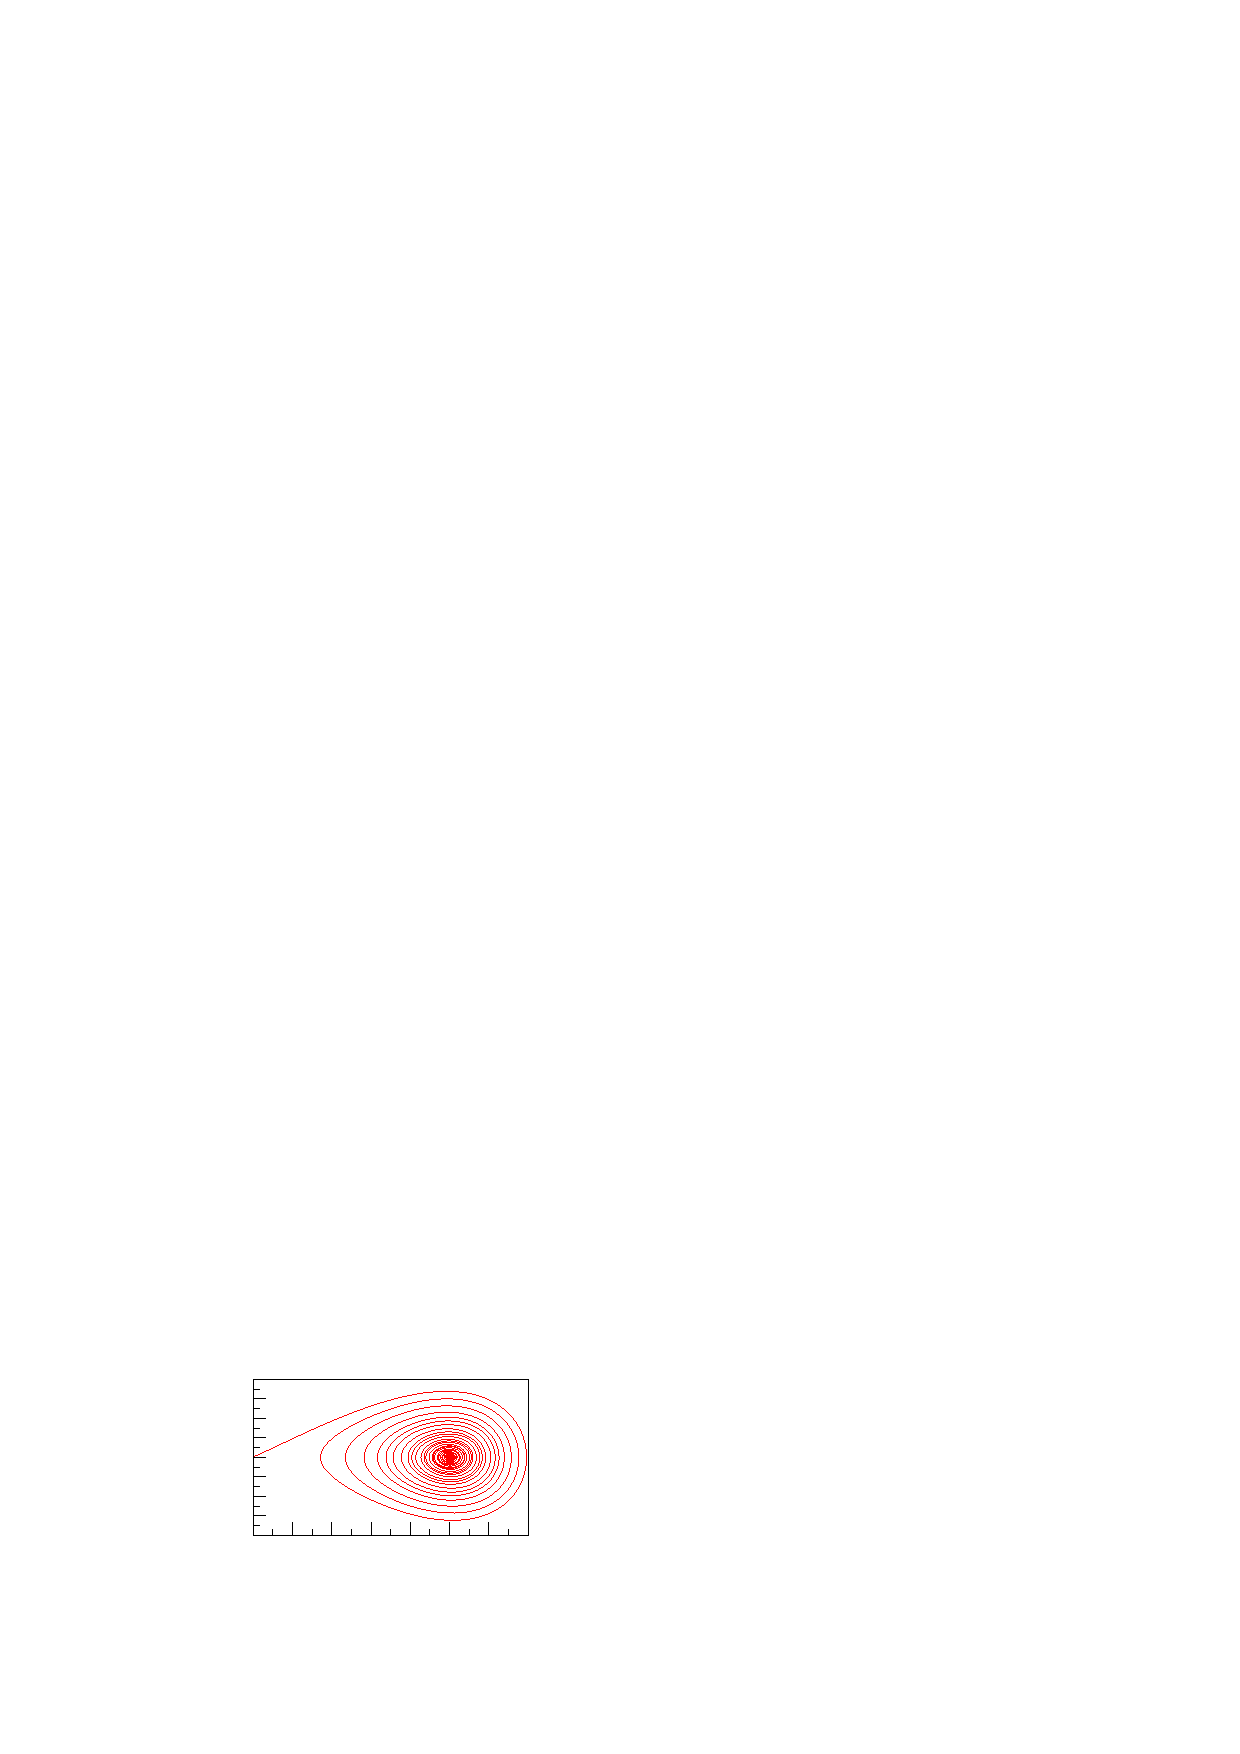
\includegraphics{Images/epslatex/phase1}%
\end{picture}%
\begingroup
\setlength{\unitlength}{0.0200bp}%
\begin{picture}(9900,5940)(0,0)%
\put(2200,1650){\makebox(0,0)[r]{\strut{}-0.8}}%
\put(2200,2117){\makebox(0,0)[r]{\strut{}-0.6}}%
\put(2200,2585){\makebox(0,0)[r]{\strut{}-0.4}}%
\put(2200,3052){\makebox(0,0)[r]{\strut{}-0.2}}%
\put(2200,3520){\makebox(0,0)[r]{\strut{} 0}}%
\put(2200,3988){\makebox(0,0)[r]{\strut{} 0.2}}%
\put(2200,4455){\makebox(0,0)[r]{\strut{} 0.4}}%
\put(2200,4923){\makebox(0,0)[r]{\strut{} 0.6}}%
\put(2200,5390){\makebox(0,0)[r]{\strut{} 0.8}}%
\put(2475,1100){\makebox(0,0){\strut{} 0}}%
\put(3418,1100){\makebox(0,0){\strut{} 0.2}}%
\put(4361,1100){\makebox(0,0){\strut{} 0.4}}%
\put(5304,1100){\makebox(0,0){\strut{} 0.6}}%
\put(6246,1100){\makebox(0,0){\strut{} 0.8}}%
\put(7189,1100){\makebox(0,0){\strut{} 1}}%
\put(8132,1100){\makebox(0,0){\strut{} 1.2}}%
\put(9075,1100){\makebox(0,0){\strut{} 1.4}}%
\put(550,3520){\rotatebox{90}{\makebox(0,0){\strut{}$y$}}}%
\put(5775,275){\makebox(0,0){\strut{}$x$}}%
\end{picture}%
\endgroup
\endinput
 \label{fig:duff_phase_1} }
\subfigure[][]{ %GNUPLOT: LaTeX picture with Postscript
\begin{picture}(0,0)%
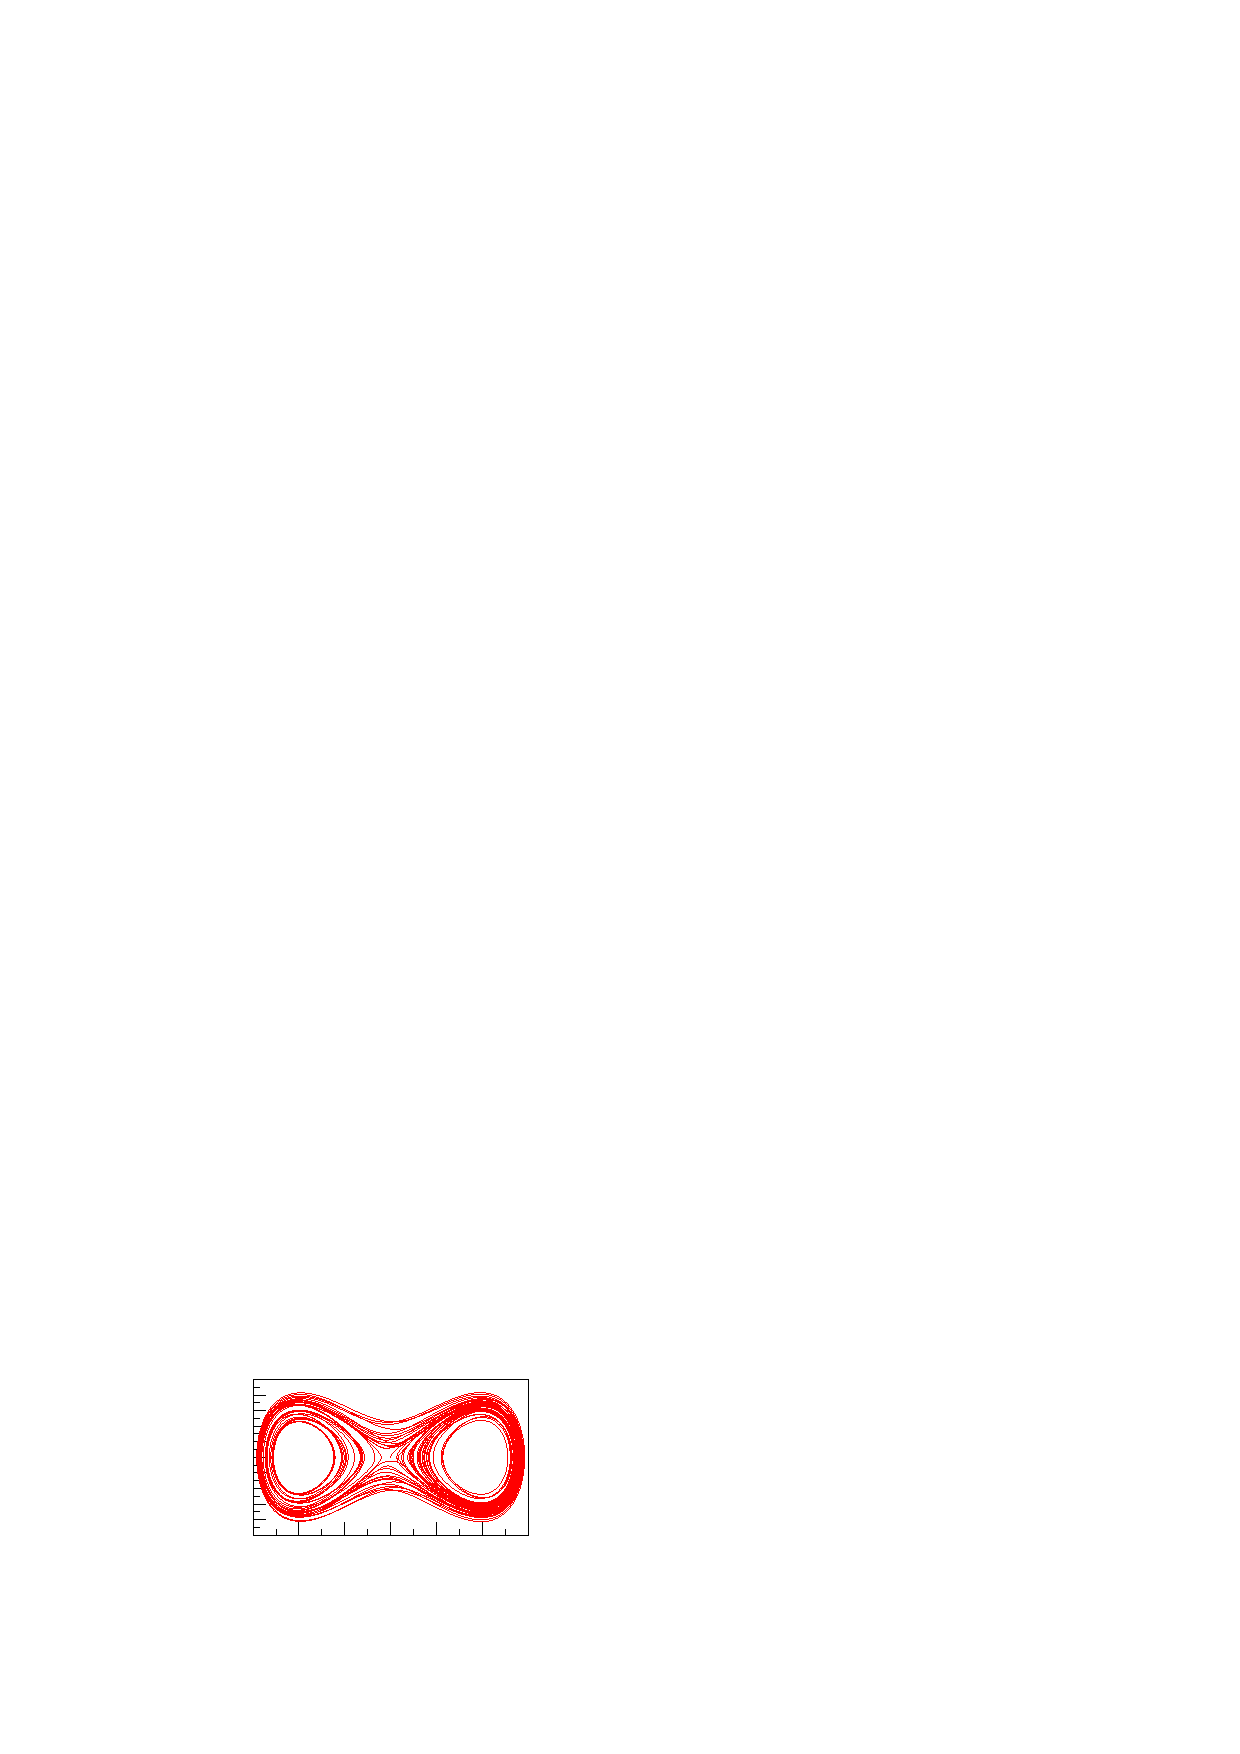
\includegraphics{Images/epslatex/phase2}%
\end{picture}%
\begingroup
\setlength{\unitlength}{0.0200bp}%
\begin{picture}(9900,5940)(0,0)%
\put(2200,1650){\makebox(0,0)[r]{\strut{}-1}}%
\put(2200,2024){\makebox(0,0)[r]{\strut{}-0.8}}%
\put(2200,2398){\makebox(0,0)[r]{\strut{}-0.6}}%
\put(2200,2772){\makebox(0,0)[r]{\strut{}-0.4}}%
\put(2200,3146){\makebox(0,0)[r]{\strut{}-0.2}}%
\put(2200,3520){\makebox(0,0)[r]{\strut{} 0}}%
\put(2200,3894){\makebox(0,0)[r]{\strut{} 0.2}}%
\put(2200,4268){\makebox(0,0)[r]{\strut{} 0.4}}%
\put(2200,4642){\makebox(0,0)[r]{\strut{} 0.6}}%
\put(2200,5016){\makebox(0,0)[r]{\strut{} 0.8}}%
\put(2200,5390){\makebox(0,0)[r]{\strut{} 1}}%
\put(2475,1100){\makebox(0,0){\strut{}-1.5}}%
\put(3575,1100){\makebox(0,0){\strut{}-1}}%
\put(4675,1100){\makebox(0,0){\strut{}-0.5}}%
\put(5775,1100){\makebox(0,0){\strut{} 0}}%
\put(6875,1100){\makebox(0,0){\strut{} 0.5}}%
\put(7975,1100){\makebox(0,0){\strut{} 1}}%
\put(9075,1100){\makebox(0,0){\strut{} 1.5}}%
\put(550,3520){\rotatebox{90}{\makebox(0,0){\strut{}$y$}}}%
\put(5775,275){\makebox(0,0){\strut{}$x$}}%
\end{picture}%
\endgroup
\endinput
 \label{fig:duff_phase_2} }
% \subfigure[][]{ \input{Images/epslatex/poincare1.tex} \label{fig:duff_poincare_1} }
% \subfigure[][]{ \input{Images/epslatex/poincare2.tex} \label{fig:duff_poincare_2} }
\end{center}
\caption[Regular and chaotic Duffing oscillators]{\baselineskip=1.0\normalbaselineskip%
The trajectories and phase diagrams of a regular and irregular Duffing oscillator.}
\label{fig:poincare_duff}
\end{figure} % 
%
\begin{figure}[h!tbp]
\begin{center}
\subfigure[][]{\input{Images/epslatex/u1.tex}\label{fig:u1} }
\subfigure[][]{%GNUPLOT: LaTeX picture with Postscript
\begin{picture}(0,0)%
\includegraphics{Images/epslatex/u2.eps}%
\end{picture}%
\begingroup
\setlength{\unitlength}{0.0200bp}%
\begin{picture}(9900,6480)(0,0)%
\put(2475,1650){\makebox(0,0)[r]{\strut{}-500}}%
\put(2475,2126){\makebox(0,0)[r]{\strut{} 0}}%
\put(2475,2601){\makebox(0,0)[r]{\strut{} 500}}%
\put(2475,3077){\makebox(0,0)[r]{\strut{} 1000}}%
\put(2475,3552){\makebox(0,0)[r]{\strut{} 1500}}%
\put(2475,4028){\makebox(0,0)[r]{\strut{} 2000}}%
\put(2475,4503){\makebox(0,0)[r]{\strut{} 2500}}%
\put(2475,4979){\makebox(0,0)[r]{\strut{} 3000}}%
\put(2475,5454){\makebox(0,0)[r]{\strut{} 3500}}%
\put(2475,5930){\makebox(0,0)[r]{\strut{} 4000}}%
\put(2750,1100){\makebox(0,0){\strut{}-10}}%
\put(3383,1100){\makebox(0,0){\strut{}-8}}%
\put(4015,1100){\makebox(0,0){\strut{}-6}}%
\put(4648,1100){\makebox(0,0){\strut{}-4}}%
\put(5280,1100){\makebox(0,0){\strut{}-2}}%
\put(5913,1100){\makebox(0,0){\strut{} 0}}%
\put(6545,1100){\makebox(0,0){\strut{} 2}}%
\put(7178,1100){\makebox(0,0){\strut{} 4}}%
\put(7810,1100){\makebox(0,0){\strut{} 6}}%
\put(8443,1100){\makebox(0,0){\strut{} 8}}%
\put(9075,1100){\makebox(0,0){\strut{} 10}}%
\put(550,3790){\rotatebox{90}{\makebox(0,0){\strut{}$u_{2}$}}}%
\put(5912,275){\makebox(0,0){\strut{}$t$}}%
\end{picture}%
\endgroup
\endinput
\label{fig:u2} }
\subfigure[][]{%GNUPLOT: LaTeX picture with Postscript
\begin{picture}(0,0)%
\includegraphics{Images/epslatex/x0.eps}%
\end{picture}%
\begingroup
\setlength{\unitlength}{0.0200bp}%
\begin{picture}(9900,6480)(0,0)%
\put(2200,1650){\makebox(0,0)[r]{\strut{} 0}}%
\put(2200,2185){\makebox(0,0)[r]{\strut{} 0.2}}%
\put(2200,2720){\makebox(0,0)[r]{\strut{} 0.4}}%
\put(2200,3255){\makebox(0,0)[r]{\strut{} 0.6}}%
\put(2200,3790){\makebox(0,0)[r]{\strut{} 0.8}}%
\put(2200,4325){\makebox(0,0)[r]{\strut{} 1}}%
\put(2200,4860){\makebox(0,0)[r]{\strut{} 1.2}}%
\put(2200,5395){\makebox(0,0)[r]{\strut{} 1.4}}%
\put(2200,5930){\makebox(0,0)[r]{\strut{} 1.6}}%
\put(2475,1100){\makebox(0,0){\strut{}-10}}%
\put(3135,1100){\makebox(0,0){\strut{}-8}}%
\put(3795,1100){\makebox(0,0){\strut{}-6}}%
\put(4455,1100){\makebox(0,0){\strut{}-4}}%
\put(5115,1100){\makebox(0,0){\strut{}-2}}%
\put(5775,1100){\makebox(0,0){\strut{} 0}}%
\put(6435,1100){\makebox(0,0){\strut{} 2}}%
\put(7095,1100){\makebox(0,0){\strut{} 4}}%
\put(7755,1100){\makebox(0,0){\strut{} 6}}%
\put(8415,1100){\makebox(0,0){\strut{} 8}}%
\put(9075,1100){\makebox(0,0){\strut{} 10}}%
\put(550,3790){\rotatebox{90}{\makebox(0,0){\strut{}$x_{0}$}}}%
\put(5775,275){\makebox(0,0){\strut{}$t$}}%
\end{picture}%
\endgroup
\endinput
\label{fig:x0} }
\subfigure[][]{\input{Images/epslatex/y0.tex}\label{fig:y0} }
\subfigure[][]{\input{Images/epslatex/x1.tex}\label{fig:x1} }
\subfigure[][]{%GNUPLOT: LaTeX picture with Postscript
\begin{picture}(0,0)%
\includegraphics{Images/epslatex/y1}%
\end{picture}%
\begingroup
\setlength{\unitlength}{0.0200bp}%
\begin{picture}(9900,6480)(0,0)%
\put(2200,1650){\makebox(0,0)[r]{\strut{}-1}}%
\put(2200,2506){\makebox(0,0)[r]{\strut{}-0.5}}%
\put(2200,3362){\makebox(0,0)[r]{\strut{} 0}}%
\put(2200,4218){\makebox(0,0)[r]{\strut{} 0.5}}%
\put(2200,5074){\makebox(0,0)[r]{\strut{} 1}}%
\put(2200,5930){\makebox(0,0)[r]{\strut{} 1.5}}%
\put(2475,1100){\makebox(0,0){\strut{}-10}}%
\put(4125,1100){\makebox(0,0){\strut{}-5}}%
\put(5775,1100){\makebox(0,0){\strut{} 0}}%
\put(7425,1100){\makebox(0,0){\strut{} 5}}%
\put(9075,1100){\makebox(0,0){\strut{} 10}}%
\put(550,3790){\rotatebox{90}{\makebox(0,0){\strut{}$y_{1}\left(t,t_{0}^{}\right)$}}}%
\put(5775,275){\makebox(0,0){\strut{}$t$}}%
\end{picture}%
\endgroup
\endinput
\label{fig:y1} }
\caption[First order approximations of modified Duffing oscillator]{\baselineskip=1.0\normalbaselineskip%
Components of the first order perturbations for homoclinic orbits for the modified Duffing oscillator over a suitable range. In these diagrams $\delta=1$, $\omega=1$ and $\gamma=1$. In subfigures~\ref{fig:x1} and~\ref{fig:y1} when $t_{0}=0.1$ is in red, $t_{0}=0.2$ is in dark blue, $t_{0}=0.3$ is in light blue and $t_{0}=0.4$ is in purple. At the points $t=t_0$ the curves are discountinuous.}
\label{fig:new_duffing}
\end{center}
\end{figure}